
\algblockdefx[Operation]{Operation}{EndOperation}%
[2]{{\bf operation} $\act{#1}$(#2)}%
{{\bf end operation}}
\algblockdefx[Procedure]{Procedure}{EndProcedure}%
[2]{{\bf procedure} $\act{#1}$(#2)}%
{{\bf end procedure}}
\algblockdefx[Receive]{Receive}{EndReceive}%
[2]{{\bf Upon receive} (#1)$_{\text{ #2 }}${\bf from} $q$}%
{{\bf end receive}}

In this section, we describe \ares{}.
%As opposed to its predecessors \cite{LS02, AKMS09}, \ares{} 
In the presentation of  \ares{} algorithm
%, compared to its predecessors \cite{LS02, AKMS09}, 
we decouple the reconfiguration service from the shared memory emulation, by utilizing
the DAPs presented in Section \ref{ssec:dap}. This allows \ares{},
to handle both the reorganization of the servers that host the data, as well as utilize 
a different atomic memory implementation per configuration. It is also important to 
note that \ares{} adopts a client-server architecture and separates the reader, writer 
and reconfiguration processes from the server processes that host the object data.
 %
\kmk{More precisely, \ares{} algorithm comprises  of three major components: $(i)$ The reconfiguration protocol which consists
 of invoking, and subsequently installing new configuration via the \act{reconfig} operation by recon clients.
 $(ii)$ The read/write protocol for executing the \act{read} and \act{write} operations invoked by readers and writers.
 $(iii)$ The implementation of the DAPs for each installed configuration 
 that respect 
 %the consistency properties  (
 Property~\ref{property:dap} and 
 which are used by the 
 %on top of which the 
 \act{reconfig}, \act{read} and 
 \act{write} operations. } %are implemented.}
 
%In the rest of the section we first provide the specification of the reconfiguration mechanism used in \ares{},
%along with the properties that this service offers. Then, we discuss the implementation of read and write 
%operations and how they utilize the reconfiguration service to ensure atomicity even in cases where 
%read/write operations are concurrent with reconfiguration operations. The read and write operations are 
%described in terms of the data access primitives presented in Section \ref{ssec:dap} and we show that
%if the DAP properties are satisfied then \ares{} preserves atomicity. This allows \ares{} to deploy the transformation
%of any atomic read/write algorithm \nn{in terms of the presented DAPs} without compromising consistency. 

%show the correctness of \ares{} when using 
% the DAP of two different algorithms: (1) of the classic replication algorithm \mwABD{}, and (2) of the new algorithm \flexCAS{} that uses erasure codes. 
%We show that \ares{} preserves atomicity independently from the DAP it utilizes. 

%will show how our reconfiguration
%service can be combined with 
%%implementations of {\sc get} and {\sc put} primitives 
%a replication algorithm to implement atomic read/write objects,
%and finally we will show how to modify the {\sc get} and {\sc put}
%primitives of the replicated algorithm to allow the use of erasure 
%codes without violating safety.
 
%\paragraph{State Variables} Here we describe the state variables in the writers, readers and servers.
%
%\myemph{Servers}:~ $\tg{}\in\N \times\wSet,~v\in V$

%\paragraph{Preliminaries:} Before proceeding with the description of the algorithm we provide 
%the data types we use and the external services we assume. 
%%Here we describe the state variables in the writers, readers and servers.


%From the definition we can conclude that if a the consensus instance $\consensus{c}$ 
%%runs over a configuration $c$ and 
%decides a value $c_k$ 
%then any subsequent invocation of $Cons[c]$ over the same configuration $c$ will decide $c_k$.  

\subsection{Implementation of the Reconfiguration Service.}
%\vspace{-.5em}
\label{ssec:recbox} 
In this section, we describe the reconfiguration service in \ares{}.
The service relies on an underlying sequence of configurations (\kmk{already proposed or installed 
by \act{reconfig} operations}), 
%which can be  
%\textit{updated} by reconfiguration clients and \textit{read} by any client in $\idSet$. 
%Our service revolves around the idea that configurations are stored in the form of
%Configurations are stored 
%The set of configurations proposed by various reconfiguration clients, by invoking reconfiguration operations, are stored  in the form of 
in the from of a  ``distributed list'', which we refer to as the \myemph{global configuration sequence (or list)} $\gseq$. 
Conceptually, $\gseq$ represents
%The data type \myemph{configuration sequence}  
an ordered list of pairs $\langle c, status \rangle$, where $c$ is a configuration identifier ($ c \in \confSet$),  
 and a binary state variable $status \in \{F, P\}$
%. The variable $status$ associated with $c$,
that denotes whether $c$ is \myemph{finalized} ($F$) or is still \myemph{pending} ($P$). 
\nn{Initially,  $\gseq$ contains a single element, say $\tup{c_0, F}$, 
	%denote the first element of $\gseq$,
	 which is known to every participant in the service.}

\nn{ To facilitate the creation of $\gseq$, each}
server in $\servers{c}$ maintains a local variable $nextC  \in  \{\confSet \cup \{\bot\}\}\times\{P,F\}$, %(to point to the next configuration in $\gseq$), $nextC \in  \{\confSet \cup \{\bot\}\}\times\{P,F\}$,
which is used to point to the configuration that follows $c$ in $\gseq$. 
Initially, at any server  $nextC = \tup{\bot, F}$. Once $nextC$ it is set to a value %in $\confSet$ 
it is never altered.  As we show below, 
at any point in the execution of~\ares{} and in any configuration $c$, the 
%set of values, that are not equal to $\bot$, stored in 
$nextC$ variables of the non-faulty servers  in $c$ that are not equal to $\bot$ agree, i.e., 
 $\{s.nextC : s \in \servers{c} \wedge s.nextC\neq \bot\}$ is either empty of has only one element.
%We use the notation $|\cseq{seq}|$ to denote the length of a sequence.

 Clients discover the configuration that follows a $\tup{c,*}$
in the sequence by contacting a subset of servers in $\servers{c}$ and collecting their $nextC$ variables. 
%Each server in $\servers{c}$ has a variable $nextC$ (one for each configuration), $nextC \in  \{\confSet \cup \{\bot\}\}\times\{P,F\}$,
%which is used to point to the configuration that follows $c$ in $\gseq$. 
Every client in $\idSet$ maintains a local variable $cseq$ that is expected to  be some subsequence of 
$\gseq$.  Initially, at every client the value of  $cseq$ is $\tup{c_0,F}$.
We use the notation $\cseq{x}$ (a caret over some name) to denote state variables
that assumes values from the domain $\{\confSet \cup \{\bot\}\}\times\{P,F\}$. %\nn{[NN: By element you mean the pair here?]} 
 %or $\cseq{config}$, or $\cseq{c}$, etc.

Reconfiguration clients may introduce new configurations,
each associated with a unique configuration identifier from $\confSet$.
 Multiple clients may concurrently attempt to introduce 
different configurations for same next link  in  $\gseq$.
\ares{} uses consensus to resolve such conflicts: 
\nn{a subset of servers in $\servers{c}$, in each configuration $c$,  
%collectively 
implements a distributed consensus service (such as 
  Paxos~\cite{L98}, RAFT~\cite{Raft}) , denoted by $\consensus{c}$. }
%that runs on a subset of servers in the configuration $c$.

%
%We implement $\gseq$ as follows. 
%In any configuration $c$, every server in $\servers{c}$ has a configuration sequence variable $cseq$, 
%initially $\tup{c_0,F}$, where new configurations can be added to the end of the list. 
%Every server in $\servers{c}$ has a variable $nextC$, $nextC \in  \{\confSet \cup \{\bot\}\}\times\{P,F\}$. Initially, at any server  $nextC = \tup{\bot, F}$, and once it is set to a value %in $\confSet$ 
%it is never altered. For any 
%$c \in \confSet$,  at any point in time, all the values of $nextC$, such that $nextC \neq \tup{\bot,F}$, in the processes  in $\servers{c}$ are the same.


% Our service revolves around the idea that configurations are stored in the form of a “distributed linked
%list“ (similar to a block-chain), which we refer to as the \textit{global configuration sequence}, denoted by $\gseq$.
%
%, where reconfig clients introduce new configurations.
%In our setting, we assume throughout an execution of \ares, every configuration is attempted to be reconfigured at most once.
 %
% Multiple  clients may attempt concurrently to introduce 
%a different configuration for the same index $i$ in the $\gseq$.
%\ares{} uses consensus to resolve such conflicts. In particular, each configuration $c$  
%is associated with an external consensus service, denoted by $\consensus{c}$,  
%that runs on a subset of servers in the configuration $c$.
%We use the data-type  $status\in\{F,P\}$, corresponding to a configuration, say $c$,  to denote whether  $c$ is \myemph{finalized} ($F$) 
%or is still \myemph{pending} ($P$).
%Each reconfigurer may change the system configuration by introducing a new configuration identifier. 
%So essentially, $\gseq$
%%The data type \myemph{configuration sequence}  
%is an array  of pairs $\langle c, status \rangle$, where $c \in \confSet$  and $status \in \{F, P\}$. We denote each such pair %\nn{[NN: By element you mean the pair here?]} 
%by the caret over a variable name, e.g., $\cseq{x}$ or $\cseq{config}$, or $\cseq{c}$, etc.
 
% \nnrev{At any point in an execution of \ares{},}{For any  
% $c_i, c_j \in \confSet$, we say that $c_i$ points to $c_j$ %(or there link 
%% (denote as $c_i \rightarrow c_j$)
% %\nn{[NN: This notation conflicts with the before notation we used in the definition of atomicity in the model. Maybe we can remove the definition there to save space and just point the reader to Lynch's book.]} 
% in $\gseq$, in a state $\state$  if at that point in the execution where a   server in $\servers{c_j}$
% %\nn{[NN: I think here does not have to be a majority of servers. A server sets its variable only after consensus has decided]} in $\servers{c_i}$ 
% has $nextC = c_j$. 

%To link a configuration $c_1$ 
%to a configuration $c_2$, a process needs to \textit{inform} (by setting the state variable $nextC$ to $c_2$) 
% we set a state variable ($nextC$) to $c_2$, 
%Each link of the list, say from configuration $c_1$ to $c_2$ is created by setting the $nextC$ state variable to $c_2$,  
%a proper subset of servers in $\servers{c_1}$ for the existence of $c_2$. 
%When a subsequent process wants to retrieve the configuration that follows 
%$c_1$ by contacting a proper set of servers in $\servers{c_1}$.
%Servers maintain a different $nextC$ variable for each configuration, which 
%initially, 
%at any server that are added  the variable $nextC$ 
%is set to $\bot$, as each server may participate in multiple configurations. 
% Each reconfiguration client starts with an initial non-empty configuration sequence $cseq$. In order, for the 
% reconfiguration operation to be successful it is necessary that the initial $cseq$ has a configuration whose $status$ is finalized.
% Each reconfigurer attempts to install a new 
% configuration $c$ in the system whenever it invokes a  $\act{reconfig}(c)$ action. 
 
%Briefly, the $\act{add-config}$ action atomically appends the local configuration sequence of the
%$\recBox$, say $cseq_{box}$, by $\tup{c,P}$ and returns the resulting configuration sequence through the $\act{add-config-ack}$
%action. The \act{read-config} returns $cseq_{box}$ through the associated 
%ack action, and finally the $\act{finalize-config}$ action marks the elements with indices between $start$ and $end$ in $cseq_{box}$
%with $\tup{*,F}$.
The  reconfiguration service consists of two major components: 
$(i)$ \myemph{sequence traversal}, responsible of discovering a  recent configuration in $\gseq$, and 
$(ii)$  \myemph{reconfiguration operation} that installs new configurations in $\gseq$.  

\begin{algorithm*}[!ht]
	%\hrule \F
	\begin{algorithmic}[2]
		\begin{multicols}{2}	{\small
				\Procedure{read-config}{$seq$}
				\State $\mu = \max(\{j: seq[j].status = F\})$	\label{line:readconfig:final}
				%\State $\nu = |cseq|$
				\State $\cseq{c} \gets seq[\mu]$ %.cfg$
				%\State {\bf send} $(\text{{\sc read-config}}, recon_i)$ to each   $s\in \bigcup_{\mu \leq i \leq \nu} \servers{currCfg}$
				\While{$\cseq{c} \neq \bot$}
				%\State {\bf send} $(\text{\act{read-config}}, recon_i)$ to each $s\in \servers{c}$
				%\State {\bf until}  $\forall j,  \mu \leq j\leq \nu$  $\wedge$  
				%$\exists\quo{},  \quo{} \in \quorums{cseq[j].cfg}$ s.t. $ \forall s\in\quo{},  recon_i$  receives $cseq_s$ from $s$ 
				%\State {\bf until} $\exists\quo{},  \quo{}\in\quorums{c}$ s.t. $\forall s\in\quo{}, recon_i$  receives $nextC_s$ from $s$
				%\State $ell \gets \max_{cseq'\text{ received }}(|cseq'|)$
				\State $ \cseq{c}' \gets$\act{get-next-config}$(\cseq{c}.cfg)$ 
				\If{$ \cseq{c}' \neq\bot$} 
				\State $\mu\gets \mu+1$				\label{line:readconfig:increment}
				\State $seq[\mu] \gets \cseq{c}'$	\label{line:readconfig:assign}
				\State \act{put-config}$(seq[\mu-1].cfg, seq[\mu])$ 	\label{line:readconfig:put}
				\State $\cseq{c} \gets seq[\mu]$ \label{line:newconfig:assign}
				\EndIf
				\EndWhile
				\State {\bf return} $seq$
				\EndProcedure
				
				\Statex
				
				\Procedure{get-next-config}{$c$}
				\State {\bf send} $(\text{{\sc read-config}})$ to each $s\in \servers{c}$
				\State {\bf until} $\exists\quo{},  \quo{}\in\quorums{c}$ s.t. $rec_i$ receives $nextC_s$ from $\forall s\in\quo{}$
				\If{$\exists s\in \quo{}\text{ s.t. } \status{nextC_s} = F$} 
					\State {\bf return} $nextC_s$
				\ElsIf{$\exists s\in \quo{}\text{ s.t. } \status{nextC_s} = P$} 
						\State {\bf return} $nextC_s$
					\Else
						\State {\bf return} $\bot$
				\EndIf 
				\EndProcedure
				
				\Statex
				
				\Procedure{put-config}{$c, nextC$}
				\State {\bf send} $(\text{{\sc write-config}}, nextC)$ to each $s\in \servers{c}$
				\State {\bf until} $\exists\quo{},  \quo{}\in\quorums{c}$ s.t. $rec_i$ receives {\sc ack} from $\forall s\in\quo{}$
				\EndProcedure	
		}\end{multicols}	
	\end{algorithmic}
	%\hrule \B
	\caption{Sequence traversal at each process $\pr\in\idSet$ of algorithm \ares.}
	\label{algo:parser}
	\vspace{-1em}
\end{algorithm*}

\myparagraph{Sequence Traversal.} 
Any \act{read/write/reconfig} operation $\op$ utilizes the sequence traversal mechanism  to discover the 
latest state of the global configuration sequence, as well as to ensure that such a state is discoverable
by any subsequent operation $\op'$. 
%
\kmk{See Fig.~\ref{fig:reconfig} for an example execution in the 
case of a reconfig operation.} \nn{In a high level, a client starts by 
collecting the $nextC$ variables from a quorum of servers in a configuration $c$,
such that $\tup{c,F}$ is the last  
finalized configuration in that client's local $cseq$ variable (or $c_0$ 
if no other finalized configuration exists). If any server $s$
returns a $nextC$ variable such that $nextC.cfg\neq\bot$,
then the client $(i)$ adds $nextC$ in its local $cseq$, $(ii)$ propagates $nextC$ 
in a quorum of servers in  $\servers{c}$, and $(iii)$ 
repeats this process in the configuration $nextC.cfg$. 
The client terminates when all servers reply with $nextC.cfg=\bot$.} 
%
More precisely, the sequence parsing consists of three actions (see Alg.~\ref{algo:parser}):  
%$(i)$ \act{get-next-config}(), to discover the next configuration, 
%$(ii)$ \act{put-config}(), which \nn{writes back $nextC$ to a quorum of servers},
%%makes sure the at least a majority of the servers in a configuration has $nextC$ to the same configuration 
%and  $(iii)$ \act{read-config}(), which finally returns \nn{the updated configuration sequence}. %a recent configuration in $\gseq$.
%%All three actions are part of the \textit{read/write/reconfig} operations. 
%We do present their specification and implementations 
%% here and we just 
%%refer to them during the description of the \textit{read/write/reconfig} operations. In high level, a $\act{read-config}$ 
%%action starts with a given configuration sequence and tries to append it with the latest installed configurations, a 
%%$\act{put-config}$ action propagates a configuration id to the servers of a given configuration, and lastly a
%%$\act{get-next-config}$ returns the configuration that follows a given configuration. More precisely the three 
%%actions are implemented 
%as follows (Alg.~\ref{algo:parser}):
%%\begin{itemize}
%%	\item 

\act{get-next-config}$(c)$:
	The action $\act{get-next-config}$ returns the configuration that follows $c$ in $\gseq$.
	During  \act{get-next-config}$(c)$, a client sends {\sc read-config}
	messages to all the servers in $\servers{c}$, and waits for replies containing $nextC$
	%. Once a server receives such a message responds with the value  of its $nextC$ variable. 
	%Once it receives replies 
	from a quorum in $\quorums{c}$. If there exists a reply with 
	%that contains a 
	$nextC.cfg\neq\bot$ 
	the action returns $nextC$; otherwise it returns $\bot$.  
	
%	\item 
\act{put-config}$(c, c')$:  
The $\act{put-config}(c, c')$ action propagates $c'$ to a quorum of servers in $\servers{c}$.
     During the action, the client  sends $( \mbox{{\sc write-config}}, c')$ messages,  
	to  the servers in $\servers{c}$ and waits for each server $s$ in some quorum $Q\in\quorums{c}$ to respond. 
	
%	\item 
\act{read-config}$(seq)$: 
	A $\act{read-config}(seq)$  sequentially traverses the installed configurations 
	%in $\gseq$ \nnrev{and  attempts  to set the status of the last configuration in $\gseq$ to $F$}{
	in order to discover the latest state of the sequence $\gseq$. 
	%This action accepts a configuration sequence $seq$ as an input and 
	%traverses the ``links'' between configurations to establish the latest form of the global configuration sequence. 
	At invocation, the client starts with the 
	last finalized configuration $\tup{c, F}$ in the given $seq$ (Line A\ref{algo:parser}:\ref{line:readconfig:final}), 
	%say $c=\config{\cseq{c_{\mu}}}$, 
	and  enters a loop to  traverse  $\gseq$ by  invoking  $\act{get-next-config}(c)$, which returns the next configuration, say $\cseq{c}'$.
	While  $\cseq{c}' \neq \bot$, then: (a) $\cseq{c}'$ is appended at the end of the sequence $seq$;
	(b) a $\act{put-config}(c, \cseq{c}')$ is invoked to inform a quorum of servers in $\servers{c}$  to update the value of their
 $nextC$ variable to $\cseq{c}'$;
	and (c) variable $c$ is set to $\config{\cseq{c}'}$. %and $c’ = \act{get-next-config}(c_r)$. 
%The	$\act{put-config}(c, c_r)$ action is done in order to ensure that subsequent operations will retrieve a link to configuration $c_r$ from $\servers{c}$. 
	%the see the links as the current reconfiguration operations.
	If $\cseq{c}' = \bot$ the loop terminates and the action  \act{read-config} returns $seq$. 
%\end{itemize}


\begin{algorithm*}[!h]
	%\hrule \F
	\begin{algorithmic}[2]
		\begin{multicols}{2}{\small
				\State at each reconfigurer $rec_i$ 
				\State {\bf State Variables:}
				%\State  $\tg{}\in\N^+\times\wSet,~v\in V$
				\State  $cseq[] s.t. cseq[j]\in\confSet\times\{F,P\}$ with members:
				%\State $cseq[j].cfg\in\confSet$, the configuration identifier
				%\State $cseq[j].status\in\{F,P\}$, the configuration status 
				\State {\bf Initialization:} 
				\State $cseq[0] = \tup{c_0,F}$
				%\State $tg{}\gets \tup{0,\bot}, v \gets \bot, cseq[0] = \tup{c_0,F}$
				
				\Statex		
				
				\Operation{reconfig}{c} 
				%\State $wCounter\gets wCounter+1$
				\If {$c \neq \bot$} 		\label{line:install:valid}
				\State $cseq\gets$\act{read-config}$(cseq)$
				\State $cseq \gets \text{\act{add-config}}(cseq, c)$ %\Comment{Read the latest configuration sequence}
				\State $\text{\act{update-config}}(cseq)$
				\State $cseq\gets\text{\act{finalize-config}}(cseq)$
				\EndIf
				\EndOperation
				
				%				\Statex
				%				
				%				
				%				\Procedure{read-config}{$seq$}
				%				\State $\mu = \max(\{j: seq[j].status = F\})$	\label{line:readconfig:final}
				%				%\State $\nu = |cseq|$
				%				\State $c \gets seq[\mu].cfg$
				%				%\State {\bf send} $(\text{{\sc read-config}}, recon_i)$ to each   $s\in \bigcup_{\mu \leq i \leq \nu} \servers{currCfg}$
				%				\While{$c \neq \bot$}
				%				%\State {\bf send} $(\text{\act{read-config}}, recon_i)$ to each $s\in \servers{c}$
				%				%\State {\bf until}  $\forall j,  \mu \leq j\leq \nu$  $\wedge$  
				%				%$\exists\quo{},  \quo{} \in \quorums{cseq[j].cfg}$ s.t. $ \forall s\in\quo{},  recon_i$  receives $cseq_s$ from $s$ 
				%				%\State {\bf until} $\exists\quo{},  \quo{}\in\quorums{c}$ s.t. $\forall s\in\quo{}, recon_i$  receives $nextC_s$ from $s$
				%				%\State $ell \gets \max_{cseq'\text{ received }}(|cseq'|)$
				%				\State $nextC \gets$\act{read-next-config}$(c)$ 
				%				\If{$nextC.cfg\neq\bot$} 
				%				\State $\mu\gets \mu+1$				\label{line:readconfig:increment}
				%				\State $seq[\mu] \gets nextC$	\label{line:readconfig:assign}
				%				\State \act{put-config}$(seq[\mu-1].cfg, seq[\mu])$
				%				\State $c \gets seq[\mu].cfg$
				%				\Else
				%				\State $c \gets \bot$
				%				\EndIf
				%				\EndWhile
				%				\State {\bf return} $seq$
				%				\EndProcedure
				
				\Statex	
				\Procedure{add-config}{$seq$, $c$}
				%\State $\mu\gets\max(\{j: cseq[j].status = F\})$
				%\State $\nu \gets |cseq|$
				%\State $\mu'\gets\max(\{j: cseq'[j].status = F\})$
				\State $\nu \gets |seq|$
				\State $c' \gets seq[\nu].cfg$
				\State $d\gets \consensus{c'}.propose(c)$
				\State $seq[\nu+1]\gets \tup{d,P}$ 				\label{line:addconfig:assign}
				\State $\act{put-config}(c', \tup{d,P})$		\label{line:addconfig:put}
				\State  {\bf return} $seq$
				\EndProcedure
				
				\Statex
				
				\Procedure{update-config}{$seq$}
				\State $\mu\gets\max(\{j: seq[j].status = F\})$
				\State $\nu\gets |seq|$ 
				
				\State $M \gets \emptyset$
				\For{$i=\mu:\nu$}
				\State $\tup{t, v}  \gets \dagetdata{\config{seq[i]}}$
				\State $M  \gets M \cup  \{ \tup{\tg{}, v} \}$ \label{line:reconfig:max}
				\EndFor
				\State $\tup{\tg{},v} \gets \max_{t} \{ \tup{t, v}: \tup{t, v} \in M\}$
				%\State $\tup{\tg{},v} \gets \text{\act{get-data}}(cseq, \mu, \nu)$
				\State $seq[\nu].\act{put-data}(\tup{\tg{},v})$
				\EndProcedure
				
				\Statex	
				
				
				\Procedure{finalize-config}{$seq$}
				\State $\nu = |seq|$
				\State $seq[\nu].status \gets F$	\label{line:status:finalize}
				\State $\act{put-config}(seq[\nu-1].cfg, seq[\nu])$
				\State \textbf{return} $seq$ 
				\EndProcedure
				
				%				\Statex	
				%				
				%				\Procedure{read-next-config}{$c$}
				%				\State {\bf send} $(\text{{\sc read-config}})$ to each $s\in \servers{c}$
				%				\State {\bf until} $\exists\quo{},  \quo{}\in\quorums{c}$ s.t. $rec_i$ receives $nextC_s$ from $\forall s\in\quo{}$
				%				\If{$\exists s\in \quo{}\text{ s.t. } nextC_s.cfg\neq\bot$} 
				%				\State {\bf return} $nextC_s$
				%				\Else
				%				\State {\bf return} $\bot$
				%				\EndIf 
				%				\EndProcedure
				%				
				%				\Statex
				%				
				%				\Procedure{put-config}{$c, cfgPtr)$}
				%				\State {\bf send} $(\text{{\sc write-config}}, cfgPtr)$ to each $s\in \servers{c}$
				%				\State {\bf until} $\exists\quo{},  \quo{}\in\quorums{c}$ s.t. $rec_i$ receives {\sc ack} from $\forall s\in\quo{}$
				%				\EndProcedure
				
				%				\Statex
				%				
				%				\Procedure{get-data}{$c$}
				%				%	\State {\bf send} $(\text{{\sc query}},\rdr)$ to every server $s\in \bigcup_{cseq[i]}members(\qs_{cseq[i].conf})$
				%				\State {\bf send} $(\text{{\sc query}})$ to each  $s\in \servers{c}$
				%				\State {\bf until}    $\exists \quo{}, \quo{}\in\quorums{c}$ s.t. 
				%				\State\TT $rec_i$ receives $\tup{t_s,v_s}$ from $\forall s\in\quo{}$ 
				%				\State $t_{max} \gets \max(\{t_s : recon_i \text{ received } \tup{t_s,v_s} \text{ from } s \})$
				%				\State {\bf return} $\{\tup{t_s,v_s}:t_s=t_{max} \wedge ~rec_i \text{ received } \tup{t_s,v_s} \text{ from } s\}$
				%				\EndProcedure
				%				
				%				\Statex	
				%				
				%				\Procedure{put-data}{$c, \tup{\tg{},v})$}
				%				\State {\bf send} $(\text{{\sc write}}, \tup{\tg{},v})$ to each $s \in \servers{c}$
				%				\State {\bf until} $\exists \quo,  \quo \in \quorums{c}$ s.t. $rec_i$ receives {\sc ack} from $\forall s\in\quo{}$
				%				\EndProcedure
				
				%\Statex \red{we need the server part for the reconfigurer}
				
		}\end{multicols}	
	\end{algorithmic}
	%\hrule \B
	\caption{Reconfiguration protocol of algorithm \ares.}
	\label{algo:reconfigurer}
	\vspace{-1em}
\end{algorithm*}

\begin{algorithm*}[!ht]
	%\hrule \F
	\begin{algorithmic}[2]
		\begin{multicols}{2}{\small
			\State at each server $s_i$ in configuration $c_k$
			\State{\bf State Variables:}
			\State  $\tg{}\in\N \times\wSet$, initially, $\tup{0,\bot}$
			\State $v\in V$, intially, $\bot$
			\State $nextC\in \confSet\times \{P,F\}$, initially $\tup{\bot,P}$
			%\State  $msgType\in\{~seen\subseteq\mathcal{V}\cup\{w\}$	
			%\State{\bf Initialization:}
			%\State $\tg{}\gets \tup{0,\bot}, v \gets \bot$
			
			\Statex
			
			\Receive{{\sc read-config}}{$s_i,c_k$}
			\State send $nextC$ to $q$
			\EndReceive
			
			\Statex
			
			\Receive{{\sc write-config}, $cfgT_{in}$}{$s_i,c_k$}
			\If{$nextC.cfg=\bot~\vee~nextC.status=P$} \label{line:server:finalize}
			\State $nextC\gets cfgT_{in}$
			\EndIf
			\State send {\sc ack} to $q$
			\EndReceive
			
%			\Statex	
%			
%			\Receive{{\sc query-tag}}{$s_i,c_k$} %\Comment{Called upon reception of a message}
%				\State $\act{handle-get-tag(c_k)}$
%				%\State send $\tg{}$ to $q$
%			\EndReceive
%			
%			\Statex
%			
%			\Receive{{\sc query}}{$s_i,c_k$}
%				\State $\act{handle-get-data(c_k)}$
%				%\State send $\tup{\tg{}, v}$ to $q$
%			\EndReceive
%			
%			\Statex
%			
%			\Receive{{\sc write}, $\tup{\tg{in}, v_{in}}$}{$s_i,c_k$}
%				\State $\act{handle-put-data(c_k)}$
%%				\If {$\tg{in}> \tg{}$} 	\label{line:server:tg-comparison}
%%					\State  $\tup{\tg{},v}\gets \tup{\tg{in},v_{in}}$ \label{line:server:update}
%%				\EndIf
%%				\State  send  {\sc ack} to $q$ 	\label{line:server:reply}
%			\EndReceive
%	
			
		}\end{multicols}	
	\end{algorithmic}
	%\hrule \B
	\caption{Server protocol of algorithm \ares.}
	\label{algo:server}
	\vspace{-1em}
\end{algorithm*}

\myparagraph{Reconfiguration operation.}
%Consensus is used at the heart of reconfiguration, in order to establish the order on the proposed configurations. 
%	In each configuration $c$, a consensus protocol runs on the servers in  $\servers{c}$, and any reconfiguration client can  
%	propose a configuration $c'\neq c$ on the consensus instance of configuration $c$.
%In particular, 
A reconfiguration operation $\act{reconfig}(c)$, $c \in \mathcal{C}$,  invoked by any reconfiguration client 
$rec_i$, attempts to append $c$ to $\gseq$. \kmk{The set of server processes in $c$ are not a part of any other configuration different 
from $c$.} \nn{In a high-level, $rec_i$ first executes a sequence traversal to discover 
the latest state of $\gseq$. Then it attempts to add the new configuration $c$, at the end of the 
discovered sequence by proposing $c$ in the consensus instance of the last configuration in the sequence. 
The client accepts and appends the decision of the consensus instance (that might be different than $c$).
Then it attempts to transfer the latest value of the read/write object to the latest installed configuration. 
Once the information is transferred, $rec_i$ finalizes the last configuration in its local sequence and 
propagates the finalized tuple to a quorum of servers in that configuration.}
%
The operation consists of four phases, executed consecutively by $rec_i$ (see Alg.~\ref{algo:reconfigurer}): 
%$(i)$  $\act{read-config}$, reads the recent global configuration sequence;  
%$(ii)$ $\act{add-config}$, attempts to append a new configuration $c$;
% $(iii)$ $\act{update-config}$, scans for the most recent object value (w.r.t. their tags)
%  in the set of configurations in its local state variable $cseq$, and writes this value to the most recent 
%  configuration in $cseq$, $(iv)$ $\act{finalize-config}$, sets the $status$ component 
%  of the last tuple  in the local $cseq$ to $F$. More precisely:

$\act{read-config}(seq)$: The phase $\act{read-config}(seq)$ at $rec_i$, reads the recent global configuration 
sequence as described in the sequence traversal. 
%The phase $\act{read-config}(seq)$ at $rec_i$, 
% reads the recent global configuration sequence 
% %client of the system 
% starting with  some initial guess\footnote{An external directory service can be use to get the information on an active configuration. For  more information on this see ~\cite{aguileratutorial}.} of $seq$. %\nn{[NN: Maybe we can add a footnote saying that a guess can be provided by a DNS like service?]}
%% Beginning from the last finalized configuration $c_{\mu}$ in $cseq$, 
%% %that is in $status$ as $P$ , 
%% $\act{read-config}(cseq)$  traverses  the links of the reconfiguration list successively discovering the new configuration from a current one by reading the $nextC$ variable, via request-response phase,   from a quorum of servers from one configuration to another. 
%%The traversal of a link from $c_1$ to $c_2$ is done by calling function $\act{read-next-config}(c_1)$, which essentially request the $nextC$ variables from a quorum of servers in $c_1$ and returns a valid configuration (i.e. $c_2 \neq \bot$) if at least one of the responses return a non-$\bot$, otherwise, it returns $\bot$.
%%Following each $\act{read-next-config}(c_1)$ call that returns a valid configuration, $rec_i$ sends the pair 
%%$\tup{c_1, F}$ to the servers in $c_1$, and awaits acknowledgements from a quorum in $c_1$. The servers
%%receiving $\tup{c_1, F}$ sets is $nextC$ to $\tup{c_1, F}$ and sends an acknowledgement to $rec_i$. This
%%write-back is done in order to ensure that subsequent  reconfig operations can see the links as the current reconfiguration operations. 
%As described above, the $\act{read-config}$ action completes the traversal by returning a possibly 
%extended configuration sequence to $cseq$.

$\act{add-config}(seq, c)$: The $\act{add-config}(seq, c)$ attempts to append a new configuration $c$ to the end of  \nnrev{$\gseq$}{$seq$ (client's view of $\gseq$)}. Suppose the last configuration in $seq$ is $c'$ (with status either $F$ or $P$), then in order to decide the 
most recent configuration, $rec_i$ invokes $\consensus{c'}.propose(c)$, on the consensus object associated with configuration $c'$. 
Let  $d\in\confSet$ be the configuration identifier decided by the consensus service.
If $d \neq c$,  this  implies that another (possibly concurrent) reconfiguration operation, invoked  by a reconfigurer $rec_j\neq rec_i$, proposed and succeeded $d$  as the configuration to follow $c'$.
%imply that $d$ is a another configuration already added into the global configuration sequence, possibly due to another reconfiguration operation by some reconfiguration client.
 In this case, $rec_i$  adopts $d$ as it own propose configuration, by  adding $\tup{d, P}$ to the end of its local $cseq$ (entirely ignoring $c$),
 using the operation $\act{put-config}(c', \tup{d, P})$, and returns the extended configuration $seq$.
 %and continues executing the remaining phases of the reconfiguration operation. 
 %Next, via the 
\remove{
\nn{[NN: We have talked about the action below so we can remove this description.]}

$\act{put-config}(c', \tup{d, P})$:
Once the $cseq$ is appended, $rec_i$ invokes the 
action $c'.\act{put-config}(\tup{d, P})$, to send $\tup{d,P}$ to a quorum of servers in $\servers{c'}$. 
%and awaits
% responses from a quorum; and upon receiving 
%such a message sets the value $nextC$ to $\tup{d, P}$ and responds with an acknowledgement to $rec_i$. 
Finally, $cseq$ is updated to the extended configuration sequence $seq'$ returned by the $\act{add-config}$ action. 
}

$\act{update-config}(seq)$:
Let us denote by $\mu$ the index of the last configuration in the local sequence $cseq$, at $rec_i$, 
such that its corresponding status is 
$F$; and $\nu$ denote the last index of $cseq$.  Next $rec_i$ invokes $\act{update-config}(cseq)$, which 
gathers the tag-value pair corresponding to 
the maximum tag in each of the configurations in $\cseq{cseq[i]}$ for $\mu \leq i \leq \nu$,
and transfers that pair to the configuration that was added by the $\act{add-config}$ action. 
The $\act{get-data}$ and $\act{put-data}$ DAPs are used to transfer the value of the object to the new configuration, 
and they are implemented \nnrev{respectively}{with respect} to the 
%atomic algorithm that is used in each of the 
configuration that is accessed. 
%During the  execution of the procedure  $\act{get-data}(cseq[i])$, $rec_i$ sends requests the tag-value  to all servers  in  $cseq[i]$ and awaits responses from a quorum.  
Suppose $\tup{t_{max}, v_{max}}$  is the tag value pair corresponding to the highest tag among the responses from all the $\nu - \mu + 1$ configurations. Then, 
 $\tup{t_{max}, v_{max}}$  is written to the configuration $d$ via the invocation of  
 $\config{\cseq{cseq[\nu]}}.\act{put-data}(\tup{\tg{max},v_{max}})$.
 
 {\footnotesize
	\begin{figure}[!t]
		\begin{center}
			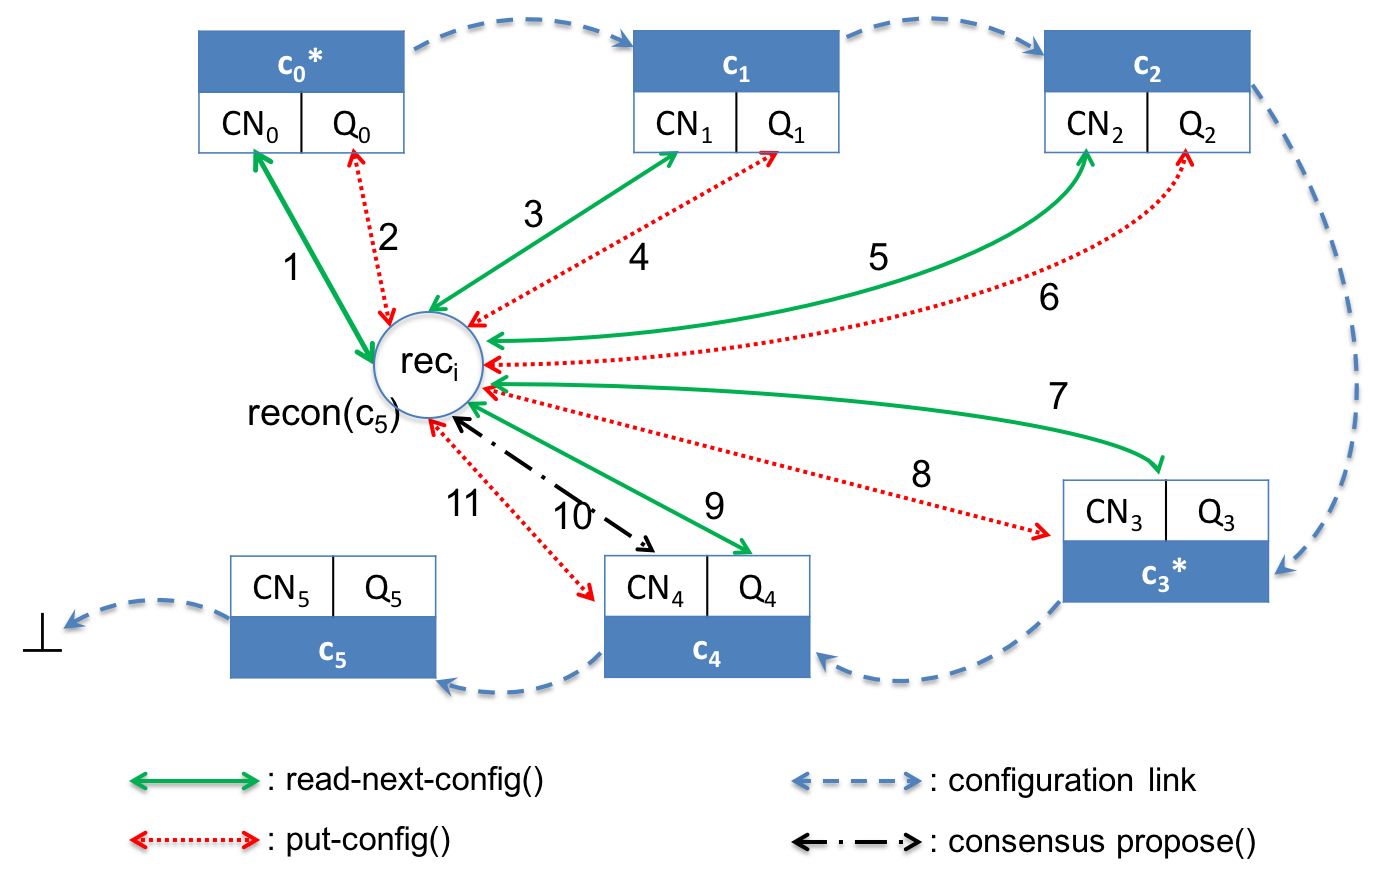
\includegraphics[width=0.5\textwidth]{ReconFig-v4.png}
			\caption{Illustration of an execution of the reconfiguration steps.}
			\label{fig:reconfig}
		\end{center}
		\vspace{-2.3em}
	\end{figure}
}

\sloppy$\act{finalize-config}(cseq)$:
Once the tag-value pair is transferred, in the last phase of the reconfiguration operation,  $rec_i$ executes %the procedure call 
$\act{finalize-config}(cseq)$, 
%during which, it 
to update the status of the last configuration in $cseq$, say $d = \config{\cseq{cseq[\nu]}}$, to $F$. 
%and writes to a quorum of the penultimate configuration of $cseq$, i.e., $cseq[\nu -1]$ and completes the reconfiguration operation.
The reconfigurer $rec_i$ informs a quorum of servers in the previous configuration $c=\config{\cseq{cseq[\nu-1]}}$, i.e.  in some $Q \in \quorums{c}$, 
about the change of status, by executing the $\act{put-config}(c, \tup{d,F})$ action. 

\myparagraph{Server Protocol.}
Each server  responds to requests from clients (Alg.~\ref{algo:server}). 
A server waits for \nnrev{five}{two} types of messages: {\sc read-config} and  {\sc write-config}.
% {\sc query}, {\sc query-tag}, and {\sc write} messages. 
When a {\sc read-config } message is received for a particular configuration $c_k$, then the server returns $nextC$ variables of the servers in $\servers{c_k}$. %\nn{[NN:again this notation]} 
A {\sc write-config} message attempts to update the $nextC$ variable of the server with a particular tuple $cfgT_{in}$.
A server changes the value of its local $nextC.cfg$ in two cases: (i) $nextC.cfg=\bot$, or (ii) $\status{nextC}= P$.

Fig.~\ref{fig:reconfig} 
%\nn{[NN: this is wrong numbering. probably has to do with the numbering of algorithms]} 
illustrates an example execution of a reconfiguration operation
$\act{recon}(c_5)$. %and the traversal of a concurrent write operation. 
In this example, the reconfigurer $rec_i$ goes through a number of configuration queries (\act{read-next-config})
before it reaches configuration $c_4$ in which a quorum of servers replies with $nextC.cfg=\bot$. 
There it proposes $c_5$ to the consensus object of $c_4$ ($\consensus{c_4}.propose(c_5)$ on arrow 10), and 
once $c_5$ is decided, $\act{recon}(c_5)$ completes after executing $\act{finalize-config}(c_5)$.



%\red{Recent reconfiguration attempts with some 
% configuration is are attempted to be added to the end of the list as the last recent link $c_{\nu}$ to $c$.  The status variable $status$ for such a configuration is set to $P$ in a quorum of servers.
%%
% A reconfig client $rc$, executing $recon(rc)$ executes three main steps. During the first step (  Line XXX $cseq \leftarrow read-config(cseq))$, $rc$ traverses the links of the reconfigurations successively discovering the new configuration from a current one by reading the $nextC$ variable  from a quorum of servers in the current configuration. Note the initial configuration is the final 
% configuration in $cseq$ such that its status is in $F$.
% }
%\blue{
%The reconfiguration protocol aims to install a new configuration and transfer the knowledge from previous configurations
%to the newly installed configuration. In particular, when a reconfiguration is invoked, the reconfigurer issues an 
%$\act{add-config}(c)$ action to the $\recBox$ attempting to add its proposed configuration to the configuration sequence
%stored in the $\recBox$. The $\recBox$ atomically appends its local configuration sequence and returns the appended 
%configuration sequence, $cseq$, to the reconfigurer. Notice that the newly added configuration $c$ appears as the last 
%element of the sequence $cseq[|cseq|]=\tup{c,P}$.
%%
%We assume a consensus service that can be executed by the members of a configuration. In each configuration
%$k$ we run a consensus instance to agree on the configuration id of $k+1$. The servers maintain a $cseq$ 
%array and are queried for the configuration identifier in a particular index.  
%}
%\paragraph{State Variables} Here we describe the state variables in the writers, readers and servers.
%
%\myemph{Servers}:~ $\tg{}\in\N \times\wSet,~v\in V$
%		%$cseq[~]$, array with elements in $\confSet\times\{F,P\}$ with members:
%		%	$cseq[i].conf\in\confSet$, the configuration identifier
%		%	 $cseq[i].status\in\{F,P\}$, the pending or finalized status 


%
%\begin{algorithm}[!ht]
%	\caption{$\rdIOA{\text{ReconBox}}{}$ Automaton: Signature of the ReconBox service} \label{ioa:reconbox-sig}
%	\begin{algorithmic}[2]
%		\begin{multicols}{2}{\small
%%				
%%				\State {\bf Data Types:}
%%				\State\T $\msgSet \subseteq \{\text{\sc{read},\sc{write}\}}\times\tup{\Nat\times\valSet}\times\Nat$
%%				
%%				\Statex
%%				
%				\Part{Signature}{ \label{line:reconbox-sig}
%				%	\State {\bf Input:}
%					\State\T $\act{add-config}(c), c\in \confSet$
%					\State\T $\act{read-config}$
%					\State\T $\act{finalize-config}(start, end)$, ~$start,end\in \N^+$
%					
%				%	\Statex
%					
%				%	\State {\bf Output:}
%					%\State\T $\act{add-config-ack}(cseq)$, $cseq[i]\in\confSet\times\{F,P\}, 0\leq i \leq |cseq|$
%					%\State\T $\act{read-config-ack}(cseq)$, ~$cseq[i]\in\confSet\times\{F,P\}, 0\leq i \leq |cseq|$
%					%\State\T $\act{finalize-config-ack}$ 
%	%				\State {\bf Internal:}
%				}\EndPart \label{line:reconbox-sig-end}
%		}\end{multicols}
%	\end{algorithmic}	
%\end{algorithm}


%Let the  $\act{recon}(c_5)$ operation be invoked by a reconfigurer $rec_i$. 
%%and the write operation by %$\act{read-next-config}(c_3)$ step executed by 
%%some writer $w$.
%During the first round of communication (arrow 1 in figure), $rec_i$ queries a quorum of servers in $c_0$ (noted by $Q_0$) and finds
%out $c_1$ as the next configuration (i.e. the link $c_0$ to $c_1$ in the global configuration sequence),
%via $\act{read-next-config}(c_0)$ 
%. %(arrow heads 1 and 2). 
%That is, at least a single server in the quorum $Q_0$ replied with $nextC$, where $nextC.cfg=c_1$ to $rec_i$.
%Next, in the second round of communication, $rec_i$ writes back $c_1$ to some 
%quorum in $c_0$ via the step $\act{put-config}(c_0, c_1)$ (see arrow 2).  In the subsequent steps $rec_i$ 
%communicates with configurations $c_1$, $c_2$ and $c_3$, in a similar manner like the above two communication rounds for $c_0$ (see arrows 3-8). 
%However,  in the first communication round with servers in  $c_4$, $rec_i$ discovers that all servers in a quorum of 
%servers in $c_4$ replied with 
%%the $nextC$ returned from
%$nextC$ such that $nextC.cfg=\bot$ (arrow 9). In other words, a link from $c_4$ to another configuration is not discovered by $rec_i$. As a result, 
%$rec_i$ proposes $c_5$ to the consensus object in $c_4$, i.e.,  it invokes $\consensus{c_4}.propose(c_5)$ (arrow 10) and 
%$\consensus{c_4}.propose(c_5)$ returns $c_5$, i.e., $c_5$ is decided as the next configuration after $c_4$. Next, $rec_i$ writes $c_5$ to a 
%quorum of servers in $c_4$ via the $\act{put-config}(c_4, c_5)$ (arrow 11), and completes the operation after executing $\act{finalize-config}(c_5)$. 
%Writer $w$  
%%happens to 
%starts its operation 
%%and the 
%with an initial guess of $cseq$ 
%%it starts with has 
%that contains $c_3$ as the last 
%configuration with 
%%its corresponding 
%a $status$ as $F$. With the two rounds of communication  (arrow heads a, b, c and d) with the servers in $c_3$,
%$w$ discovers $c_4$. However, similar communication rounds with the servers in $c_4$ returns $\bot$, i.e.,  $\act{read-next-config}(c_4)$ returns $\bot$.

%To install a new configuration the reconfigurer has to execute the following steps: (i) attempt to add the 
%new configuration, (ii) transfer the latest data to the new configuration, and (iii) mark the new configuration 
%as finalized. Below we describe each action separately: 
%\begin{itemize}
%	\item \myemph{add-config}: The \act{add-config}(c) action attempts to add the proposed configuration $c$ at 
%	the end of the current configuration sequence. In brief, a new configuration is added by following these steps:
%	(i) perform a read-config at a guessed configuration and by following the finalized configurations try to establish 
%	a sequence with a single finalized and a set of pending configs, (ii) propose $c$ by running consensus on the 
%	last discovered configuration (trying to establish the immediately next config), and (iii) once you receive the 
%	decided configuration propagate the new sequence to the latest config.
%\end{itemize}
%
%The read-config operation needs to have a mechanism to discover the latest finalized configuration. 
%Thus when we try to read the configuration sequence from 
%
%The reconfigurer finalizes the last configuration in its $cseq$ as this is the last configuration he added. 
%To do so he first sets the status of the last configuration, say $c$, to $F$ and propagates its local $cseq$ 
%to the following configurations in sequence: (i) contacts a quorum in $c$, and then (ii) contacts a quorum in 
%$cseq[\mu]$, where $\mu$ is the last finalized configuration of $cseq$ (before $c$). This way we ensure that



%\subsection{\ares{} over a Replicated Atomic Read/Write Object}
%\label{ssec:replicated} 

%To demonstrate that the reconfiguration service provides sufficient properties to implement 
%a reconfigurable atomic read/write object, we first present  an algorithm 
%where the distributed object is replicated among the set of servers. 
%The read and write operations (Algorithms \ref{algo:writer} and \ref{algo:reader}) are similar
%to the two phase classic algorithm of \cite{ABD96}, when they are not concurrent with a reconfiguration operation. 


\begin{algorithm*}[!ht]
	%\hrule \F
	\begin{algorithmic}[2]
		\begin{multicols}{2}{\small
				\Part{Write Operation}
				\State at each writer $w_i$ 
				%\State {\bf State Variables:}
				%\State  $\tg{},\tg{max}\in\N^+\times\wSet,~v\in V, terminate\in\{true,false\}$
				%\State  $cseq[~]$, array with elements in $\confSet\times\{F,P\}$ with members:
				%\State\T $cseq[i].conf\in\confSet$, the configuration identifier
				%\State\T $cseq[i].status\in\{F,P\}$, the pending or finalized status 
				%\State {\bf Initialization:} 
				%\State $\tg{}\gets \tup{0,w_i}$
				%\State $v \gets \bot$
				%\State $cseq[0] = \tup{c_0,F}, terminate={\bf false}$
				\State {\bf State Variables:}
				%\State  $\tg{}\in\N^+\times\wSet,~v\in V$
				\State  $cseq[] s.t. cseq[j]\in\confSet\times\{F,P\}$ with members:
				%\State\T $cseq[j].cfg\in\confSet$, the configuration identifier
				%\State\T $cseq[j].status\in\{F,P\}$, the configuration status 
				\State {\bf Initialization:} 
				\State $cseq[0] = \tup{c_0,F}$
				
				\Statex		
				
				\Operation{write}{$val$}, $val \in V$ 
				%\State $wCounter\gets wCounter+1$
				\State $cseq\gets$\act{read-config}($cseq$)  \label{line:writer:readconfig} %\Comment{Read the latest configuration sequence}
				\State $\mu\gets\max(\{i: cseq[i].status = F\})$ \label{line:writer:lastfin}
				\State $\nu\gets |cseq|$ 
				\For{$i=\mu:\nu$}
				\State $\tg{max} \gets \max(\config{cseq[i]}.\act{get-tag}(), \tg{max})$  \label{line:writer:max}
				\EndFor
				\State $\tup{\tg{},v} \gets \tup{ \tup{\tg{max}.ts+1, \wrt_i}, val}$ \label{line:writer:increment}
				\State $done \gets false$
				\While{{\bf not} $done$} \label{line:writer:whilebegin}
				\State $\config{cseq[\nu]}.$\act{put-data}$(\tup{\tg{},v})$ \label{line:writer:prop}
				\State $cseq\gets$\act{read-config}($cseq$)
				\If{$|cseq| = \nu$}
				\State $done \gets  true$
				\Else
				\State $\nu\gets |cseq|$ \label{line:writer:whileend}
				\EndIf
				\EndWhile
				\EndOperation
				\EndPart
				
				\Part{Read Operation}
				\State at each reader $\rdr_i$ 
				\State {\bf State Variables:}
				\State  $cseq[] s.t. cseq[j]\in\confSet\times\{F,P\}$ with members:
				%			\State\T $cseq[j].cfg\in\confSet$, the configuration identifier
				%			\State\T $cseq[j].status\in\{F,P\}$, the configuration status 
				\State {\bf Initialization:} 
				\State $cseq[0] = \tup{c_0,F}$
				
				\Statex
				
				\Operation{read}{ } 
				%\State $wCounter\gets wCounter+1$
				\State $cseq\gets$\act{read-config}($cseq$)  \label{line:reader:readconfig}%\Comment{Read the latest configuration sequence}
				\State $\mu\gets\max(\{j: cseq[j].status = F\})$ \label{line:reader:lastfin}
				\State $\nu\gets |cseq|$ 
				\For{$i=\mu:\nu$} \label{line:rw:getdata:start}
				\State $\tup{\tg{},v} \gets \max(\config{cseq[i]}.\act{get-data}(), \tup{\tg{},v})$ \label{line:reader:max}
				\EndFor \label{line:rw:getdata:end}
				\State $done\gets {\bf false}$
				\While{{\bf not} $done$}  \label{line:reader:whilebegin}
				\State $\config{cseq[\nu]}.\act{put-data}(\tup{\tg{},v})$ \label{line:reader:prop}
				\State $cseq\gets$\act{read-config}($cseq$)
				\If{$|cseq| = \nu$}
				\State $done \gets  true$
				\Else
				\State $\nu\gets |cseq|$ \label{line:reader:whileend}
				\EndIf
				\EndWhile
				\State {\bf return} $v$
				\EndOperation
				\EndPart
				
				%		\Procedure{get-tag}{$c$}
				%		%	\State {\bf send} $(\text{\act{query}},\rdr)$ to every server $s\in \bigcup_{cseq[i]}members(\qs_{cseq[i].conf})$
				%		\State {\bf send} $(\text{{\sc query-tag}})$ to each  $s\in \servers{c}$
				%		\State {\bf until}    $\exists \quo{}, \quo{}\in\quorums{c}$ s.t. 
				%		\State\TT$\wrtr_i$ receives $\tup{t_s,v_s}$ from $\forall s\in\quo{}$ 
				%		\State $t_{max} \gets \max(\{t_s : \wrtr_i \text{ received } \tup{t_s,v_s} \text{ from } s \})$
				%		\State {\bf return} $t_{max}$
				%		\EndProcedure
				%		
				%		\Statex				
				%		\Procedure{put-data}{$c, \tup{\tg{},v})$}
				%		\State {\bf send} $(\text{{\sc write}}, \tup{\tg{},v})$ to each $s \in \servers{c}$
				%		\State {\bf until} $\exists \quo,  \quo \in \quorums{c}$ s.t. $\wrtr_i$ receives {\sc ack} from $\forall s\in\quo{}$
				%		\EndProcedure
				%		
				%		
				%		\Statex
				
				%		\Procedure{read-config}{$seq$}
				%		\State $\mu = \max(\{j: seq[j].status = F\})$	\label{line:readconfig:final}
				%		%\State $\nu = |cseq|$
				%		\State $c \gets seq[\mu].cfg$
				%		%\State {\bf send} $(\text{{\sc read-config}}, recon_i)$ to each   $s\in \bigcup_{\mu \leq i \leq \nu} \servers{currCfg}$
				%		\While{$c \neq \bot$}
				%		%\State {\bf send} $(\text{\act{read-config}}, recon_i)$ to each $s\in \servers{c}$
				%		%\State {\bf until}  $\forall j,  \mu \leq j\leq \nu$  $\wedge$  
				%		%$\exists\quo{},  \quo{} \in \quorums{cseq[j].cfg}$ s.t. $ \forall s\in\quo{},  recon_i$  receives $cseq_s$ from $s$ 
				%		%\State {\bf until} $\exists\quo{},  \quo{}\in\quorums{c}$ s.t. $\forall s\in\quo{}, recon_i$  receives $nextC_s$ from $s$
				%		%\State $ell \gets \max_{cseq'\text{ received }}(|cseq'|)$
				%		\State $nextC \gets$\act{get-next-config}$(c)$ 
				%		\If{$nextC.cfg\neq\bot$} 
				%		\State $\mu\gets \mu+1$				\label{line:readconfig:increment}
				%		\State $seq[\mu] \gets nextC$	\label{line:readconfig:assign}
				%		\State \act{put-config}$(seq[\mu-1].cfg, seq[\mu])$
				%		\State $c \gets seq[\mu].cfg$
				%		\Else
				%		\State $c \gets \bot$
				%		\EndIf
				%		\EndWhile
				%		\State {\bf return} $seq$
				%		\EndProcedure
				%		
				%		\Statex		
				%		
				%		\Procedure{get-next-config}{$c$}
				%		\State {\bf send} $(\text{{\sc read-config}})$ to each $s\in \servers{c}$
				%		\State {\bf until} $\exists\quo{},  \quo{}\in\quorums{c}$ s.t. $\wrtr_i$ receives $nextC_s$, $\forall s\in\quo{}$
				%		\If{$\exists s\in \quo{}\text{ s.t. } nextC_s.cfg\neq\bot$} 
				%		\State {\bf return} $nextC_s$
				%		\Else
				%		\State {\bf return} $\bot$
				%		\EndIf 
				%		\EndProcedure
				%		
				%		\Statex
				%		
				%		\Procedure{put-config}{$c, cfgPtr)$}
				%		\State {\bf send} $(\text{{\sc write-config}}, cfgPtr)$ to each $s\in \servers{c}$
				%		\State {\bf until} $\exists\quo{},  \quo{}\in\quorums{c}$ s.t. $\wrtr_i$ receives {\sc ack} from $\forall s\in\quo{}$
				%		\EndProcedure
		}\end{multicols}	
	\end{algorithmic}
	%\hrule \B
	\caption{Write and Read protocols at the clients for \ares.}
	\label{algo:writer}
	\vspace{-1em}
\end{algorithm*}
\subsection{Implementation of Read and Write operations.}
The read and write operations in \ares{} are expressed in terms of the DAP primitives  (see 
Section \ref{ssec:dap}). 
%A read  consists of  an execution of  $\act{get-data}$ primitive followed by a $\act{put-data}$ primitive,
%while a write consists of calls to $\act{get-tag}$ and  $\act{put-data}$ primitives. 
This provides the flexibility to \ares{} to use different implementation of DAP primitives in different configurations, without changing the basic structure of  \ares{}. 
At a high-level, a \act{write} (or \act{read})  operation is executed where the client: $(i)$ obtains the \textit{latest configuration sequence} by using the 
$\act{read-config}$ action of the reconfiguration service, $(ii)$ queries  the configurations, in $cseq$, starting from the last finalized configuration
to the end of the discovered configuration 
sequence, for the latest $\tup{tag,value}$ pair with a help of $\act{get-tag}$ (or $\act{get-data}$) operation \nn{as specified for each configuration}, and 
$(iii)$ repeatedly propagates  a new $\tup{tag', value'}$ pair (the largest $\tup{tag,value}$ pair)   with $\act{put-data}$ in the last configuration of its local sequence, until no additional configuration is observed. 
%Now
%{\sc get} and {\sc put} primitives 
%we  describe the execution 
In more detail, the algorithm of a  read or write operation $\pi$ is as follows (see Alg.~\ref{algo:writer}): 
%The server keeps a passive behavior and replies to any message it receives. 


%Here we present the read and write operations in more detail. 
%As we presented in Section \ref{sec:primitives}, for an algorithm to 
%preserve atomicity it needs to satisfy some properties on the 
%implementation of its {\sc get} and {\sc put} primitives. 

%Those primitives are implemented in our replication algorithm as follows:
%\begin{itemize}
%	\item {\sc get-tag}$(c)$: Send {\sc query-tag} messages to all the servers in $\servers{c}$ and wait 
%	for each server $s$ in a quorum $Q\in\quorums{q}$ to reply with its local $\tg{s}$. Find and return the 
%	maximum of those tags. 
%	\item {\sc get-data}$(c)$: Send {\sc query} messages to all the servers in $\servers{c}$ and wait 
%	for each server $s$ in a quorum $Q\in\quorums{q}$ to reply with its local $\tup{\tg{s}, v_s}$ pair. 
%	Find the maximum of those tags, say $\tg{s'}$, and return the pair received by $s'$, $\tup{\tg{s'},v_{s'}}$.
%	\item {\sc put-data}$(c, \tup{\tg{},v})$: Send {\sc write-tag} messages, along with the  $\tup{\tg{},v}$ pair, 
%	to all the servers in $\servers{c}$ and wait for each server $s$ in a quorum $Q\in\quorums{q}$ to reply with an {\sc ack}. 
%\end{itemize}


A write (or read) operation is invoked at a client  $\pr$ when line~Alg.~\ref{algo:writer}:\ref{line:writer:readconfig} %for the writer  
(resp. line~Alg.~\ref{algo:writer}:\ref{line:reader:readconfig}) is executed.  
%for reader),
At first, $\pr$ issues a $\act{read-config}$ action to obtain the latest 
introduced configuration in $\gseq$, in both operations. 
%Note that each process contains a state 
%variable $cseq$ which initially contains the initial configuration $\tup{c_0,F}$. 
%Starting with a guess, $cseq$, for the latest global configuration sequence,
%As shown in the reconfiguration service, 
%process $\pr$ queries a quorum in each configuration $\config{cseq[i]}$, for $\max(j:\status{cseq[j]}=F)\leq i \leq |cseq|$,
%to discover newly introduced and/or newly finalized configurations, during the $\act{read-config}$ action. 

%We assume that each configuration has enough active servers to allow 
%$\pr$ to make progress	even when some configuration is has been replaced 
%by a newer configuration. 
%In case a system wants to garbage collect or decommission inactive servers,
%then a service similar to DNS can be used to provide an estimate of 
%the latest finalized configuration. Notice that such a service would affect 
%the liveness and not the safety of our current implementation so we do 
%not get into details on how such a service can be implemented in this paper. 

\nn{If $\op$ is a \act{write} %(resp. Alg.~\ref{algo:writer}:\ref{line:reader:lastfin} if $\op$ is a  read), 
	$\pr$ detects the last finalized entry in $cseq$, 
	say $\mu$, and performs a $cseq[j].conf.\act{get-tag}()$ action,
	for $\mu\leq j\leq|cseq|$ (line Alg.~\ref{algo:writer}:\ref{line:writer:lastfin}). Then $\pr$ discovers the
	\textit{maximum tag} among all the returned tags ($\tg{max}$),
	and it increments the maximum tag discovered 
	(by incrementing the integer part of $\tg{max}$), generating a new tag, say $\tg{new}$. It assigns 
	$\tup{\tg{}, v}$ to $\tup{\tg{new}, val}$, where $val$ is the
	value he wants to write (Line Alg.~\ref{algo:writer}:\ref{line:writer:increment}).}

\nn{
if $\op$ is a \act{read}, 
$\pr$ detects the last finalized entry in $cseq$, 
say $\mu$, and performs a  $cseq[j].conf.\act{get-data}()$ action, 
for $\mu\leq j\leq|cseq|$ (line Alg.~\ref{algo:writer}:\ref{line:reader:lastfin}). Then $\pr$ discovers the
\textit{maximum tag-value} pair ($\tup{\tg{max},v_{max}}$) among the replies, 
and assigns $\tup{\tg{}, v}$ to $\tup{\tg{max},v_{max}}$.}

%In lines Alg.~\ref{algo:writer}:\ref{line:writer:lastfin} if $\op$ is a write (resp. Alg.~\ref{algo:writer}:\ref{line:reader:lastfin} if $\op$ is a  read), 
% $\pr$ detects the last finalized entry in $cseq$, 
%say $\mu$, and performs a $cseq[j].conf.\act{get-tag}()$ action if $\op$ is a \act{write}, or $cseq[j].conf.\act{get-data}()$ action if $\op$ is a \act{read}, 
%for $\mu\leq j\leq|cseq|$. Then $\pr$ discovers the
%maximum tag among all the returned tags ($\tg{max}$) or tag-value pairs ($\tup{\tg{max},v_{max}}$) respectively.
%%sends \textit{query} messages to all the members of each configuration $cseq[j].conf$, for $\mu\leq j\leq|cseq|$.
%%Notice that any configuration $cseq[j].cfg$,  for $\mu< j\leq|cseq|$, is in a pending state and thus $cseq[j].status = P$.
%%When the client receives replies from a quorum in each configuration $cseq[j].cfg$, it discovers the maximum 
%%$\tup{\tg{max},v_{max}}$ among those replies (Lines A\ref{algo:writer}:\ref{line:writer:max} and A\ref{algo:reader}:\ref{line:reader:max}). 
%If $\op$ is a \act{write}, $\pr$ increments the maximum tag discovered 
%(by incrementing the integer part of $\tg{max}$), generates a new tag, say $\tg{new}$, and assigns 
%$\tup{\tg{}, v}$ to $\tup{\tg{new}, val}$, where $val$ is the
%value he wants to write (Line Alg.~\ref{algo:writer}:\ref{line:writer:increment}). If $\op$ is a \act{read}, then $\pr$ assigns 
%$\tup{\tg{}, v}$ to $\tup{\tg{max},v_{max}}$, i.e.,  the maximum discovered tag-value pair.
%

Once specifying the $\tup{\tg{}, v}$ to be propagated, both reads and writes 
% if $\op$ is a read, $\pr$ 
 %does the following until no new configuration is discovered: (i) 
execute the $\config{cseq[\nu]}.\act{put-data}(\tup{\tg{}, v})$ action, where $\nu=|cseq|$, 
%to a quorum in the last configuration in $cseq$, 
followed by executing  $\act{read-config}$ action, to examine whether new configurations were 
introduced in $\gseq$. The repeat these steps until no new configuration is discovered (lines  Alg.~\ref{algo:writer}:\ref{line:writer:whilebegin}--\ref{line:writer:whileend},
or lines  Alg.~\ref{algo:writer}:\ref{line:reader:whilebegin}--\ref{line:reader:whileend}).
%retrieving a config
Let $cseq'$ be the sequence returned by the $\act{read-config}$ action. 
If $|cseq'| = |cseq|$ then no new configuration is introduced, and
the read/write operation terminates; otherwise, $\pr$ sets $cseq$ to $cseq'$ and repeats the two actions. 
Note,  in an execution of  \ares,  two consecutive $\act{read-config}$ 
operations that return $cseq'$ and $cseq''$ respectively must hold that $cseq'$ is a prefix of $cseq''$,
and hence $|cseq'|=|cseq''|$ only if $cseq' = cseq''$.  Finally, if $\pi$ is a read operation the value with the highest
tag discovered is returned to the client.

\nnfix{\myparagraph{Discussion} \ares{} shares similarities with previous algorithms like RAMBO \cite{GLS03} and 
	the framework  in \cite{spiegelman:DISC:2017}. The reconfiguration technique used in \ares{} ensures the prefix property 
	on the configuration sequence (resembling a blockchain data structure \cite{N08bitcoin}) while the array structure in RAMBO allowed 
	nodes to maintain an incomplete reconfiguration history. 
	%While in RAMBO recon operation needed to write in both the old and the new configurations due to the possible non-continuity of the 
	%known configurations in the config array, in ARES the prefix property of the configuration sequence 
	%allows each recon operation to write only to the latest configuration it discovered. 
	On the other hand, the DAP usage, 
	%enables \ares{} to be oblivious on the underlying atomic memory implementation in each configuration. This 
	exploits a different viewpoint compared to \cite{spiegelman:DISC:2017}, allowing implementations of 
	atomic read/write registers without relying on strong objects, like ranked registers \cite{GD05}.	
	%	where the authors focus to provide a general framework 
	%	for reconfigurations that led to the use of read-write-modify objects, like ranked registers \cite{GD05},
	%	for the implementation of linearizable read/write objects.  
} 

%\vspace{-0.25em}
%\label{sec:correct}
%\remove{We proceed by first introducing some definitions and notation, then by presenting some properties that are satisfied 
by the reconfiguration service in any execution, and then we show that given these properties our algorithm satisfies 
the safety (atomicity) conditions. 
%Due to space limitations the proofs of the main statements are omitted and can be found in \cite{ARES:Arxiv:2018}.
}

\remove{
\myparagraph{Notations and definitions.}
For a server $s$, we use the notation $\atT{s.var}{\state}$ to refer to the value of the state variable $var$, in $s$, at a state $\state$ of an  execution $\EX$. 
If server  $s$ crashes at a state $\state_f$ in an execution $\EX$ then $\atT{s.var}{\state}\triangleq\atT{s.var}{\state_f}$ for any state variable $var$ and for 
any state $\state$ that appears after $\state_f$ in $\EX$. 
%refers to the value of $v$ at $s$ at the state just before crashes. In other words, $\atT{s.v}{T}  \triangleq \atT{s.v}{\hat{T}}$, where $\hat{T}$ is the latest point in the execution, such that, $(a)$ $\hat{T} \leq T$ and $(b)$ $s$ is non-faulty.
 }
 
 \remove{
\begin{definition}[Tag of a configuration]  Let  $c \in \mathcal{C}$ be a configuration, $\state$ be a state in some execution $\EX$ then 
we define the tag of $c$ at state $\state$ as  
$ \atT{tag(c)}{\state} \triangleq \min_{Q \in \quorums{c}} \max_{s \in Q}~\atT{(s.tag}{\state}).$
We  drop the suffix $|_\state$, and simply denote as $tag(c)$,  when the state  is clear from the context.
\end{definition}

\begin{definition}
Let $\sigma$ be any point in an execution of \ares{} and suppose we use the notation $\cvec{\pr}{\state}$ for $ \atT{\pr.cseq}{\state}$,  i.e., the $cseq$ variable at process $p$ at the state $\state$. %be the value of a configuration sequence vector at a process $\pr$ at some state  $\st$ in an execution $\EX$. 
Then we define as $ \mu(\cvec{\pr}{\state})  \triangleq  \max\{ i : \cvec{\pr}{\state}[i].status = F\}$ 
and $ \nu(\cvec{\pr}{\state}) \triangleq |\cvec{\pr}{\state}|$, where $|\cvec{\pr}{\state}|$ is the length of the  configuration vector 
$\cvec{\pr}{\state}$. % that are not equal to $\bot$.  
\end{definition}

\begin{definition} [Prefix order]
Let $\mathbf{x}$ and $\mathbf{y}$ be any two configuration sequences. We say that $\mathbf{x}$ is a prefix of $\mathbf{y}$, denoted by 
$\mathbf{x} \preceq_p  \mathbf{y}$, if $\config{\mathbf{x}[j]}=\config{\mathbf{y}[j]}$, for all $j$ such that $\mathbf{x}[j]\neq\bot$.
\end{definition}

%In this section we analyze the properties that we can achieve through our reconfiguration algorithm. 
The first lemma shows that any two configuration sequences have the same configuration identifiers
in the same indexes. 

\begin{lemma}
\label{lem:consconf}
	For any reconfigurer $r$ that invokes an $\act{reconfig}(c)$ action in an execution $\EX$ 
	of the algorithm, If $r$ chooses to install $c$ in index $k$ of its local $r.cseq$ vector, then $r$ invokes 
	the $Cons[k-1].propose(c)$ instance over configuration $r.cseq[k-1].cfg$.
\end{lemma}

\begin{proof}
	It follows directly from the algorithm. 
\end{proof}

\begin{lemma}
	\label{lem:server:monotonic}
	If a server $s$ sets $s.nextC$ to $\tup{c,F}$ at some state $\st$ in an execution $\EX$ 
	of the algorithm, then $s.nextC = \tup{c,F}$ for any state $\st'$ that appears after $\st$ in 
	$\EX$.
\end{lemma}

\begin{proof}
	Notice that a server $s$ updates the $s.nextC$ variable for some specific configuration $c_k$ 
	in a state $st$ if: (i) $s$ did not receive any value for $c_k$ before (and thus $nextC=\bot$), or (ii) $s$ 
	received a tuple $\tup{c,P}$ and before $\st$ received the tuple $\tup{c',F}$. By Observation \ref{obs:consensus}
	$c=c'$ as $s$ updates the $s.nextC$ of the same configuration $c_k$. Once the tuple becomes equal to 
	$\tup{c,F}$ then $s$ does not satisfy the update condition for $c_k$, and hence in any state $\st'$ after $\st$
	it does not change $\tup{c,F}$.
\end{proof}

\begin{lemma}[Configuration Uniqueness]
\label{lem:unique}

	%Let $\st_1$ and $\st_2$ be any two states of an execution $\EX$ of the algorithm,
	%and $\pr, q$ two participating processes. 
	%be the state after the response action of an operation $\op_1$ from process $p$,
	%and $\st_2$ be the state after the first $\act{read-config}$ call of an operation $\op_2$ from $q$.
	For any processes $\pr, q\in \idSet$ and any states $\st_1, \st_2$ in an execution $\EX$, it must hold that 
	$\config{\cvec{\pr}{\st_1}[i]}=\config{\cvec{q}{\st_2}[i]}$,  $\forall i$ s.t. 
	$\config{\cvec{\pr}{\st_1}[i]},\config{\cvec{q}{\st_2}[i]}\neq \bot$.
\end{lemma}

\begin{proof}
	The lemma holds trivially for $\config{\cvec{\pr}{\st_1}[0]}=\config{\cvec{q}{\st_2}[0]}=c_0$. 
	So in the rest of the proof we focus in the case where $i > 0$. Let us assume 
	w.l.o.g. that $\st_1$ appears before $\st_2$ in $\EX$.
	
	According to our algorithm a process $\pr$ sets $\pr.cseq[i].cfg$ to a configuration 
	identifier $c$ in two cases: (i) either it received $c$ as the result of the consensus 
	instance in configuration $\pr.cseq[i-1].cfg$, or (ii) $\pr$ receives $\config{s.nextC} = c$ from 
	a server $s\in\servers{\config{\pr.cseq[i-1]}}$. Note here that (i) is possible only 
	when $\pr$ is a reconfigurer and attempts to install a new configuration. On the 
	other hand (ii) may be executed by any process in any operation that invokes the 
	$\act{read-config}$ action. We are going 
	to proof this lemma by induction on the configuration index. 
	

	\emph{Base case:} The base case of the lemma is when $i=1$. 
	Let us first assume that $p$ and $q$ receive $c_p$ and $c_q$, as the result of the consensus instance at $\pr.cseq[0].cfg$
	and $q.cseq[0].cfg$ respectively. By Lemma \ref{lem:consconf}, since both processes want to install a configuration 
	in $i=1$, then they have to run $Cons[0]$ instance over the configuration stored in their local $cseq[0].cfg$ variable. 
	Since $\pr.cseq[0].cfg=q.cseq[0].cfg=c_0$ then 
	both $Cons[0]$ instances run over the same configuration $c_0$ and according to Observation \ref{obs:consensus}  
	return the same value, say $c_1$. Hence $c_p=c_q=c_1$ and $\pr.cseq[1].cfg=q.cseq[1].cfg=c_1$.
	 
	 Let us examine the case now where $p$ or $q$ 
	assign a configuration $c$ they received from some server $s\in\servers{c_0}$. According to the
	algorithm only the configuration that has been decided by the consensus instance on 
	$c_0$ is propagated to the servers in $\servers{c_0}$. If $c_1$ is the decided configuration, then 
	$\forall s\in\servers{c_0}$ such that $s.nextC(c_0)\neq\bot$, it holds that $s.nextC(C_0) = \tup{c_1,*}$.
	So if $p$ or $q$ set $\pr.cseq[1].cfg$ or $q.cseq[1].cfg$ to some received configuration, then 
	$\pr.cseq[1].cfg = q.cseq[1].cfg = c_1$ in this case as well. 
	
     \emph{Hypothesis:} We assume  that 
	$\cvec{\pr}{\st_1}[k]=\cvec{q}{\st_2}[k]$  for some $k$, $k \geq 1$.
	
	%\noindent{\bf Induction Hypothesis:} 
	\emph{Induction Step:}  We need to show that the lemma holds for $i=k+1$.
	If both processes retrieve $\config{\pr.cseq[k+1]}$ and $\config{q.cseq[k+1]}$ through consensus, 
	then both $\pr$ and $q$ run consensus
	over the previous configuration. Since according to our hypothesis 
	$\cvec{\pr}{\st_1}[k]=\cvec{q}{\st_2}[k]$ then both process will receive the same
	decided value, say $c_{k+1}$, and hence $\pr.cseq[k+1].cfg=q.cseq[k+1].cfg=c_{k+1}$. Similar to the base case,
	a server in $\servers{c_k}$ only receives the configuration $c_{k+1}$ decided by the consensus instance run over $c_k$. 
	So processes 
	$\pr$ and $q$ can only receive $c_{k+1}$ from some server in $\servers{c_k}$ 
	%even if the processes update their $\pr.cseq[k+1].cfg$ or $q.cseq[k+1].cfg$ with a received 
	%configuration that will be equal to 
	so they can only assign $\pr.cseq[k+1].cfg=q.cseq[k+1].cfg=c_{k+1}$ at Line \ref{algo:reconfigurer}:\ref{line:readconfig:assign}.
	That completes the proof. 
\end{proof}


Lemma \ref{lem:unique} showed that any two operations store the same
configuration in any cell $k$ of their $cseq$ variable. It is not known however 
if the two processes discover the same number of configuration ids. In the following
lemmas we will show that if a process learns about a configuration in a cell $k$ 
then it also learns about all configuration ids for every index $i$, such that $0\leq i\leq k-1$.

\begin{lemma}
\label{lem:confmonotonic}
	In any execution $\EX$ of the algorithm , If for any process $\pr\in\idSet$, $\cvec{\pr}{\st}[i]\neq\bot$ in some state $\st$ in $\EX$,
	then $\cvec{\pr}{\st'}[i]\neq\bot$ in any state $\st'$ that appears after $\st$ in $\EX$. 
\end{lemma}

\begin{proof}
	A value is assigned to $\cvec{\pr}{*}[i]$ either after the invocation of a consensus instance, or while executing
	the $\act{read-config}$ action. Since any configuration proposed for installation cannot be $\bot$ (A\ref{algo:reconfigurer}:\ref{line:install:valid}), 
	and since there is at least one configuration proposed in the consensus instance (the one from $\pr$), then by the validity of the consensus
	service the decision will be a configuration $c\neq\bot$. Thus, in this case $\cvec{\pr}{*}[i]$ cannot be $\bot$.
	Also in the $\act{read-config}$ procedure, $\cvec{\pr}{*}[i]$ is assigned to a value different than $\bot$ according
	to Line A\ref{algo:reconfigurer}:L\ref{line:readconfig:assign}. Hence, if $\cvec{\pr}{\st}[i]\neq\bot$ at state $\st$ 
	then it cannot become $\bot$ in any state $\st'$ after $\st$ in execution $\EX$.
\end{proof}


\begin{lemma}
\label{lem:nogaps}
	Let $\st_1$ be some state in an execution $\EX$ of the algorithm. Then for any 
	process $\pr$, if $k = max\{i: \cvec{\pr}{\st_1}[i]\neq \bot\}$, then 
	$\cvec{\pr}{\st_1}[j]\neq \bot$, for $0\leq j < k$.
\end{lemma}
\begin{proof}
	Let us assume to derive contradiction that there exists $j < k$ such that 
	$\cvec{\pr}{\st_1}[j]=\bot$ and $\cvec{\pr}{\st_1}[j+1]\neq\bot$.
	Suppose w.l.o.g. that $j = k-1$ and that $\st_1$ is the state immediately 
	after the assignment of a value to $\cvec{\pr}{\st_1}[k]$, say $c_k$. 
	Since $\cvec{\pr}{\st_1}[k]\neq\bot$, then $\pr$ assigned $c_k$ to $\cvec{\pr}{\st_1}[k]$ 
	in one of the following cases: 
	(i) $c_k$ was the result of the consensus instance, or
	(ii) $\pr$ received $c_k$ from a server during a $\act{read-config}$ action.
	The first case is trivially impossible as according to Lemma \ref{lem:consconf} 
	$\pr$ decides for $k$ when it runs consensus over configuration $\config{\cvec{\pr}{\st_1}[k-1]}$. 
	Since this is equal to $\bot$, then we cannot run consensus over a non-existent set of 
	processes. 	In the second case, $\pr$ assigns $\cvec{\pr}{\st_1}[k] = c_k$  in Line A\ref{algo:parser}:\ref{line:readconfig:assign}.
	The value $c_k$ was however obtained when $\pr$ invoked $\act{get-next-config}$ on 
	configuration $\config{\cvec{\pr}{\st_1}[k-1]}$. In that action, $\pr$ sends {\sc read-config}
	messages to the servers in $\servers{\config{\cvec{\pr}{\st_1}[k-1]}}$ and waits until a quorum 
	of servers replies. Since we assigned $\cvec{\pr}{\st_1}[k] = c_k$ it means that $\act{get-next-config}$
	terminated at some state $\st'$ before $\st_1$ in $\EX$, and thus: 
	(a) a quorum of servers in $\servers{\config{\cvec{\pr}{\st'}[k-1]}}$
	replied, and (b) there exists a server $s$ among those that replied with $c_k$. 
	According to our assumption however, $\cvec{\pr}{\st_1}[k-1] = \bot$ at $\st_1$. 
	So if state $\st'$ is before $\st_1$ in $\EX$, %is the state after the response step of $\act{get-next-config}$, 
	then by Lemma \ref{lem:confmonotonic}, it follows that $\cvec{\pr}{\st'}[k-1] = \bot$. This however 
	implies that $\pr$ communicated with an empty configuration, and thus no server replied to $\pr$. 
	This however contradicts the assumption that a server replied with $c_k$ to $\pr$. 
	
	Since any process traverses the configuration sequence starting from the initial 
	configuration $c_0$, then with a simple induction we can show that 
	$\cvec{\pr}{\st_1}[j]\neq \bot$, for $0\leq j\leq k$.
\end{proof}

We can now move to an important lemma that shows that any \act{read-config} action 
returns an extension of the configuration sequence returned by any previous \act{read-config} action. 
First, we show that the last finalized configuration observed by any \act{read-config} action is at least as 
recent as the finalized configuration observed by any subsequent \act{read-config} action. 
%Using this lemma we will then show that when 

\begin{lemma}
	\label{lem:config:propagation}
	If at a state $\st$ of an execution $\EX$ of the algorithm, if $\mu(\cvec{\pr}{\st}) = k$ % = \max\{i: \cvec{\pr}{\st}[i]\neq\bot\}$
	for some process $\pr$, then for any element $0\leq j < k$, $\exists Q\in \quorums{\config{\cvec{\pr}{\st}[j]}}$
	such that $\forall s\in Q, s.nextC(\config{\cvec{\pr}{\st}[j]})= \cvec{\pr}{\st}[j+1]$. 
\end{lemma}
\begin{proof}
	This lemma follows directly from the algorithm. Notice that whenever a process assigns a value to 
	an element of its local configuration (Lines  A\ref{algo:parser}:\ref{line:readconfig:assign} and 
	A\ref{algo:reconfigurer}:\ref{line:addconfig:assign}), it then propagates this value to a quorum of the 
	previous configuration (Lines  A\ref{algo:parser}:\ref{line:readconfig:put} and 
	A\ref{algo:reconfigurer}:\ref{line:addconfig:put}). So if a process $\pr$ assigned $c_j$ to an 
	element $\cvec{\pr}{\st'}[j]$ in some state $\st'$ in $\EX$, then $\pr$ may assign a value 
	to the $j+1$ element of $\cvec{\pr}{\st''}[j+1]$ only after $\act{put-config}(\config{\cvec{\pr}{\st'}[j-1]},\cvec{\pr}{\st'}[j])$
	occurs. During $\act{put-config}$ action, $\pr$ propagates $\cvec{\pr}{\st'}[j]$ in a quorum 
	$Q\in\quorums{\config{\cvec{\pr}{\st'}[j-1]}}$. Hence, if $\cvec{\pr}{\st}[k]\neq\bot$, then $\pr$ 
	propagated each $\cvec{\pr}{\st'}[j]$, for $0<j\leq k$ to a quorum of servers $Q\in\quorums{\config{\cvec{\pr}{\st'}[j-1]}}$.
	And this completes the proof. 
%	
%	Let examine a single element $\cvec{\pr}{\st'}[j]$ that is added in the configuration vector at some state $\st'$ 
%	that appears before $\st$ in $\EX$. Whenever a configuration is assigned a process $\pr$ invokes $\act{put-config}$
%	action before adding the next configuration. According to this action, the process sends the discovered configuration
%	and sends it to a quorum of servers. As this process is repeated for every element inserted then the lemma follows. 
\end{proof}


\begin{lemma}[Configuration Prefix]
	\label{lem:prefix}
Let $\op_1$ and $\op_2$ two 
%read/write/install operations 
completed \act{read-config} actions invoked by processes $\pr_1, \pr_2\in\idSet$ 
respectively, such that $\op_1\bef\op_2$ in an execution $\EX$. Let $\st_1$ be the state after the response 
step of $\op_1$ and $\st_2$ the state after the response step 
%termination of the first $\act{read-config}$ 
of $\op_2$. Then 
$\cvec{\pr_1}{\st_1}\preceq_p\cvec{\pr_2}{\st_2}$.
\end{lemma}

\begin{proof}
	Let $\nu_1 = \nu(\cvec{\pr_1}{\st_1})$ and $\nu_2 = \nu(\cvec{\pr_2}{\st_2})$.
	By Lemma \ref{lem:unique} for any $i$ such that $\cvec{\pr_1}{\st_1}[i]\neq\bot$ and 
	$\cvec{\pr_2}{\st_2}[i]\neq\bot$, then $\config{\cvec{\pr_1}{\st_1}[i]}=\config{\cvec{\pr_2}{\st_2}[i]}$.
	Also from Lemma \ref{lem:nogaps} we know that for $0\leq j\leq \nu_1, \cvec{\pr_1}{\st_1}[j] \neq \bot$, 
	and $0\leq j\leq \nu_2, \cvec{\pr_2}{\st_2}[j] \neq \bot$. So if we can show that $\nu_1\leq \nu_2$ then the lemma follows. 
	
	Let $\mu = \mu(\cvec{\pr_2}{\st'})$ %, or simply $\mu$, 
	be the last finalized element which $\pr_2$ established in the beginning of 
	the $\act{read-config}$ action $\op_2$ (Line A\ref{algo:reconfigurer}:\ref{line:readconfig:final}) at some state $\st'$ before $\st_2$. 
	It is easy to see that $\mu\leq \nu_2$. If $\nu_1 \leq \mu$ then $\nu_1\leq \nu_2$ and 
	the lemma follows. Thus, it remains
	to examine the case where $\mu < \nu_1$. Notice that since $\op_1\bef\op_2$ then $\st_1$ appears before 
	$\st'$ in execution $\EX$. By Lemma \ref{lem:config:propagation}, we know that by $\st_1$, 
	%in all the configurations $\cvec{\pr_1}{\st_1}[j]$, for $0\leq j < \nu_1$,  
	$\exists Q\in\quorums{\config{\cvec{\pr_1}{\st_1}[j]}}$, for $0\leq j < \nu_1$,   such that 
	$\forall s\in Q, s.nextC = \cvec{\pr_1}{\st_1}[j+1]$. Since $\mu < \nu_1$, then it must be the case 
	that $\exists Q\in \quorums{\config{\cvec{\pr_1}{\st_1}[\mu]}}$ such that $\forall s\in Q, s.nextC = \cvec{\pr_1}{\st_1}[\mu+1]$.
	But by Lemma \ref{lem:unique}, we know that $\config{\cvec{\pr_1}{\st_1}[\mu]}= \config{\cvec{\pr_2}{\st'}[\mu]}$. 
	Let $Q'$ be the quorum that replies to the $\act{read-next-config}$ occurred in $\pr_2$, on configuration  $\config{\cvec{\pr_2}{\st'}[\mu]}$.
	By definition $Q\cap Q'\neq \emptyset$, thus there is a server $s\in Q\cap Q'$ that sends $s.nextC = \cvec{\pr_1}{\st_1}[\mu+1]$
	to $\pr_2$ during $\op_2$. Since $\cvec{\pr_1}{\st_1}[\mu+1]\neq\bot$ then $\pr_2$ assigns $\cvec{\pr_2}{*}[\mu+1]=\cvec{\pr_1}{\st_1}[\mu+1]$, and 
	repeats the process in the configuration $\config{\cvec{\pr_2}{*}[\mu+1]}$. Since every configuration $\config{\cvec{\pr_1}{\st_1}[j]}$, 
		for $\mu\leq j<\nu_1$, has a quorum of servers with $s.nextC$, then by a simple induction it can be shown that the process will 
		be repeated for at least $\nu_1-\mu$ iterations, and  every configuration
		$\cvec{\pr_2}{\st''}[j]=\cvec{\pr_1}{\st_1}[j]$, at some state $\st''$ before $\st_2$. 
		Thus, $\cvec{\pr_2}{\st_2}[j]=\cvec{\pr_1}{\st_1}[j]$, for $0\leq j\leq \nu_1$. Hence $\nu_1\leq\nu_2$ and the lemma follows in this case as well. 
\end{proof}

Thus far we focused on the configuration member of each element in $cseq$. As operations do get in account
the \emph{status} of a configuration, i.e. $P$ or $F$, in the next lemma we will examine the relationship of 
the last finalized configuration as detected by two operations. First we present a lemma that shows the 
monotonicity of the finalized configurations.

\begin{lemma}
	\label{lem:final:monotonic}
	Let $\st$ and $\st'$ two states in an execution $\EX$ such that $\st$ appears before $\st'$ in $\EX$.
 	Then for any process $\pr$ must hold that $\mu(\cvec{\pr}{\st})\leq \mu(\cvec{\pr}{\st'})$.  %\red{must refer to a read-config}
\end{lemma}

\begin{proof}
	This lemma follows from the fact that if a configuration $k$ is such that 
	$\status{\cvec{\pr}{\st}[k]}=F$ at a state $\st$, then $\pr$ will start any 
	future $\act{read-config}$ action from a configuration $\config{\cvec{\pr}{\st'}[j]}$
	such that $j\geq k$. But $\config{\cvec{\pr}{\st'}[j]}$ is the last finalized configuration 
	at $\st'$ and hence $\mu(\cvec{\pr}{\st'})\geq \mu(\cvec{\pr}{\st})$.
\end{proof}

\begin{lemma}  [Configuration Progress]
	\label{lem:finalconf}
	Let $\op_1$ and $\op_2$ two 
	%read/write/install operations 
	completed \act{read-config} actions invoked by processes $\pr_1, \pr_2\in\idSet$ 
	respectively, such that $\op_1\bef\op_2$ in an execution $\EX$. 
	Let $\st_1$ be the state after the response 
	step of $\op_1$ and $\st_2$ the state after the response step 
	%after the completion of $\op_1$ and $\st_2$ the state after the termination of the first $\act{read-config}$ 
	of $\op_2$. Then 
	$\mu(\cvec{\pr_1}{\st_1})\leq\mu(\cvec{\pr_2}{\st_2})$.
\end{lemma}

\begin{proof}
	By Lemma \ref{lem:prefix} it follows that $\cvec{\pr_1}{\st_1}$ is a prefix of $\cvec{\pr_2}{\st_2}$.
	Thus, if $\nu_1 = \nu(\cvec{\pr_1}{\st_1})$ and $\nu_2 = \nu(\cvec{\pr_2}{\st_2})$, $\nu_1\leq\nu_2$.
	Let $\mu_1=\mu(\cvec{\pr_1}{\st_1})$, such that $\mu_1\leq\nu_1$, be the last element in $\cvec{\pr_1}{\st_1}$,
	where $\status{\cvec{\pr_1}{\st_1}[\mu_1]} = F$. Let now $\mu_2=\mu(\cvec{\pr_2}{\st'})$, 
	be the last element which $\pr_2$ obtained in Line A\ref{algo:parser}:\ref{line:readconfig:final} 
	during $\op_2$ 
	%of the  $\act{read-config}$ action 
	such that $\status{\cvec{\pr_2}{\st'}[\mu_2]} = F$ in some state $\st'$ before $\st_2$. 
	If $\mu_2\geq\mu_1$, and since $\st_2$ is after $\st'$, then by Lemma \ref{lem:final:monotonic} 
	$\mu_2\leq \mu(\cvec{\pr_2}{\st_2})$ and hence $\mu_1\leq \mu(\cvec{\pr_2}{\st_2})$ as well. 
	
	It remains to examine the case where $\mu_2<\mu_1$. Process  $\pr_1$ 
	sets the status of $\cvec{\pr_1}{\st_1}[\mu_1]$ to $F$ in two cases: (i) either when finalizing 
	a reconfiguration, or (ii) when receiving an $s.nextC = \tup{\config{\cvec{\pr_1}{\st_1}[\mu_1]}, F}$ %with status $F$ 
	from some server $s$ during a $\act{read-config}$ action. In both cases $\pr_1$ propagates the 
	$\tup{\config{\cvec{\pr_1}{\st_1}[\mu_1]}, F}$ to a quorum of servers in  
	$\config{\cvec{\pr_1}{\st_1}[\mu_1-1]}$ before completing. We know by Lemma
	\ref{lem:prefix} that since $\op_1\bef\op_2$ then $\cvec{\pr_1}{\st_1}$ is a prefix 
	in terms of configurations of the $\cvec{\pr_2}{\st_2}$. So it must be the case 
	that $\mu_2 < \mu_1 \leq \nu(\cvec{\pr_2}{\st_2})$. Thus, during $\op_2$, %the $\act{read-config}$ action, 
	$\pr_2$ starts from the configuration at index $\mu_2$ and in some iteration 
	performs $\act{get-next-config}$ in configuration $\cvec{\pr_2}{\st_2}[\mu_1-1]$. 
	According to Lemma \ref{lem:unique}, $\config{\cvec{\pr_1}{\st_1}[\mu_1-1]} = \config{\cvec{\pr_2}{\st_2}[\mu_1-1]}$.
	Since $\op_1$ completed before $\op_2$, then it must be the case that $\st_1$ appears before 
	$\st'$ in $\EX$. However, $\pr_2$ invokes the $\act{get-next-config}$ operation in a state $\st''$
	which is either equal to $\st'$ or appears after $\st'$ in $\EX$. Thus, $\st''$ must appear after $\st_1$ in $\EX$.
	From that it follows that when the $\act{get-next-config}$ is executed by $\pr_2$ there is already 
	a quorum of servers in $\config{\cvec{\pr_2}{\st_2}[\mu_1-1]}$, say $Q_1$, that received 
	$\tup{\config{\cvec{\pr_1}{\st_1}[\mu_1]}, F}$from $\pr_1$. 
	Since, $\pr_2$ waits from replies from a quorum of servers from the same configuration, say $Q_2$, and since the 
	$nextC$ variable at each server is monotonic (Lemma \ref{lem:server:monotonic}), then there is a server $s\in \quo{1}\cap \quo{2}$, 
	such that $s$ replies to $\pr_2$ with $s.nextC = \tup{\config{\cvec{\pr_1}{\st_1}[\mu_1]}, F}$. So, 
	$\cvec{\pr_2}{\st_2}[\mu_1]$ gets $\tup{\config{\cvec{\pr_1}{\st_1}[\mu_1]}, F}$, and 
	hence $\mu(\cvec{\pr_2}{\st_2})\geq \mu_1$ in this case as well. This completes our proof.
\end{proof}

\begin{theorem}
	Let $\op_1$ and $\op_2$ two 
%read/write/install operations 
completed \act{read-config} actions invoked by processes $\pr_1, \pr_2\in\idSet$ 
respectively, such that $\op_1\bef\op_2$ in an execution $\EX$. 
Let $\st_1$ be the state after the response 
step of $\op_1$ and $\st_2$ the state after the response step 
%after the completion of $\op_1$ and $\st_2$ the state after the termination of the first $\act{read-config}$ 
of $\op_2$.
%$\cvec{\pr_1}{\st_1}$ and $\cvec{\pr_2}{\st_2}$ at two states $\st_1$ and $\st_2$ 
%in an execution $\EX$ of the algorithm  such that $\st_1$ appears before $\st_2$ in $\EX$. 
Then the following properties hold: 
\begin{enumerate}
\item [$(a)$] 
$\cvec{\pr_2}{\st_2}[i].cfg = \cvec{\pr_1}{\st_1}[i].cfg$,  for $ 1 \leq i \leq \nu(\cvec{\pr_1}{\st_1})$,
\item [$(b)$]
 %$(b)$  
 $\cvec{\pr_1}{\st_1}  \preceq_p \cvec{\pr_2}{\st_2}$, and
\item [$(c)$] 
%$(c)$  
  $\mu(\cvec{\pr_1}{\st_1}) \leq \mu(\cvec{\pr_2}{\st_2})$
  %; and 
%\item [$(d)$]  
%\nn{????$(d)$  $\cvec{\pr_2}{\st_2}[i]   = \cvec{\pr_1}{\st_1}[i]$,  for  $ 1 \leq i \leq \mu(\cvec{\pr_1}{\st_1})$????} 
\end{enumerate}
\end{theorem}

\begin{proof}
Statements $(a)$, $(b)$ and $(c)$ follow from Lemmas \ref{lem:unique}, \ref{lem:prefix}, and 
\ref{lem:final:monotonic}.
%are from  the atomic read-modify-write property of ${\recBox}.\act{add-config}(\cdot)$ 
%and $(d)$ is due to the recon client.
\end{proof}
\nn{Next we analyze the properties  satisfied by  ~\ares{}. In brief, the reconfiguration algorithm
preserves three properties in any execution: 
$(i)$ \myemph{Configuration Uniqueness}, 
$(ii)$ \myemph{Configuration 
Prefix}, and 
$(iii)$ \myemph{Configuration Progress}. Configuration Uniqueness ensures that no two different 
configurations are assigned to the same index in a configuration sequence. Configuration
prefix ensures that any \act{read-config} action 
returns an extension of the configuration sequence returned by any previous \act{read-config} action. 
Finally, the configuration progress focuses on the status of the configurations in a sequence, 
and ensures that a \act{read-config} action observes at least as recent
\myemph{finalized} configuration as any preceding \act{read-config} action. The following theorem presents formally those 
properties.}

%The first lemma shows that any two configuration sequences have the same configuration identifiers
%in the same indexes. 
%
%\begin{lemma}[Configuration Uniqueness]
%	\label{lem:unique}
%	
%	%Let $\state_1$ and $\state_2$ be any two states of an execution $\EX$ of the algorithm,
%	%and $\pr, q$ two participating processes. 
%	%be the state after the response action of an operation $\op_1$ from process $p$,
%	%and $\state_2$ be the state after the first $\act{read-config}$ call of an operation $\op_2$ from $q$.
%	For any processes $\pr, q\in \idSet$ and any states $\state_1, \state_2$ in an execution $\EX$, it must hold that 
%	$\config{\cvec{\pr}{\state_1}[i]}=\config{\cvec{q}{\state_2}[i]}$,  $\forall i$ s.t. 
%	$\config{\cvec{\pr}{\state_1}[i]},\config{\cvec{q}{\state_2}[i]}\neq \bot$.
%\end{lemma}
%
%We can now move to an important lemma that shows that any \act{read-config} action 
%returns an extension of the configuration sequence returned by any previous \act{read-config} action. 
%First, we show that the last finalized configuration observed by any \act{read-config} action is at least as 
%recent as the finalized configuration observed by any subsequent \act{read-config} action. 
%%Using this lemma we will then show that when 
%
%\begin{lemma}[Configuration Prefix]
%	\label{lem:prefix}
%	Let $\op_1$ and $\op_2$ two 
%	%read/write/install operations 
%	completed \act{read-config} actions invoked by processes $\pr_1, \pr_2\in\idSet$ 
%	respectively, such that $\op_1\bef\op_2$ in an execution $\EX$. Let $\state_1$ be the state after the response 
%	step of $\op_1$ and $\state_2$ the state after the response step 
%	%termination of the first $\act{read-config}$ 
%	of $\op_2$. Then 
%	$\cvec{\pr_1}{\state_1}\preceq_p\cvec{\pr_2}{\state_2}$.
%\end{lemma}
%
%Thus far we focused on the configuration member of each element in $cseq$. As operations do get in account
%the \myemph{status} of a configuration, i.e. $P$ or $F$, in the next lemma we will examine the relationship of 
%the last finalized configuration as detected by two operations. First we present a lemma that shows the 
%monotonicity of the finalized configurations.
%
%
%\begin{lemma}  [Configuration Progress]
%	\label{lem:finalconf}
%	Let $\op_1$ and $\op_2$ two 
%	%read/write/install operations 
%	completed \act{read-config} actions invoked by processes $\pr_1, \pr_2\in\idSet$ 
%	respectively, such that $\op_1\bef\op_2$ in an execution $\EX$. 
%	Let $\state_1$ be the state after the response 
%	step of $\op_1$ and $\state_2$ the state after the response step 
%	%after the completion of $\op_1$ and $\state_2$ the state after the termination of the first $\act{read-config}$ 
%	of $\op_2$. Then 
%	$\mu(\cvec{\pr_1}{\state_1})\leq\mu(\cvec{\pr_2}{\state_2})$.
%\end{lemma}


\begin{theorem}[Reconfiguration Properties]
	Let $\op_1$ and $\op_2$ be two 
	%read/write/install operations 
	completed \act{read-config} actions invoked by processes $\pr_1, \pr_2\in\idSet$ 
	respectively, such that $\op_1\bef\op_2$ in an execution $\EX$ of ~\ares. 
	Let $\state_1$ be the state after the response 
	step of $\op_1$ and $\state_2$ the state after the response step 
	%after the completion of $\op_1$ and $\state_2$ the state after the termination of the first $\act{read-config}$ 
	of $\op_2$.
	%$\cvec{\pr_1}{\state_1}$ and $\cvec{\pr_2}{\state_2}$ at two states $\state_1$ and $\state_2$ 
	%in an execution $\EX$ of the algorithm  such that $\state_1$ appears before $\state_2$ in $\EX$. 
	Then the following holds: 
%	\begin{enumerate}
	%	\item [$(a)$] 
	$(a)$	$\cvec{\pr_2}{\state_2}[i].cfg = \cvec{\pr_1}{\state_1}[i].cfg$,  for $ 1 \leq i \leq \nu(\cvec{\pr_1}{\state_1})$,
	%	\item [$(b)$]
		%$(b)$  
	$(b)$	$\cvec{\pr_1}{\state_1}  \preceq_p \cvec{\pr_2}{\state_2}$, and
	%	\item [$(c)$] 
		%$(c)$  
	$(c)$	$\mu(\cvec{\pr_1}{\state_1}) \leq \mu(\cvec{\pr_2}{\state_2})$
		%; and 
		%\item [$(d)$]  
		%\nn{????$(d)$  $\cvec{\pr_2}{\state_2}[i]   = \cvec{\pr_1}{\state_1}[i]$,  for  $ 1 \leq i \leq \mu(\cvec{\pr_1}{\state_1})$????} 
%	\end{enumerate}
\end{theorem}
}

%\input{ssec-correct-safety_v2.tex}

%\subsection{\ares{} Liveness}
%\label{ssec:liveness}
%\input{ssec-correct-liveness.tex}

%The propagation of the information of the distributed object in \ares{} is achieved using the $\act{get-tag}$, $\act{get-data}$, 
%and $\act{put-data}$ actions.  
Given the properties satisfied by the reconfiguration algorithm of \ares{} 
and assuming that the DAP used satisfy properties $C1$ and $C2$, as presented
in Section \ref{ssec:dap}, then  we have the following result. 

\begin{theorem}[Atomicity]
    Consider  any execution of \ares{} such that in every configuration used   the DAP primitives  satisfy  the DAP consistency properties then ~\ares{} satisfy atomicity property.
	%, given that the 
	%$\act{get-data}$, $\act{get-tag}$, and $\act{put-data}$ primitives used satisfy properties
	%\textbf{C1} and \textbf{C2} of Definition \ref{def:consistency}.
\end{theorem}

%In  \ares{},  each configuration 
%may implement the DAPs in a different way as stated below:

\begin{remark}
	Algorithm \ares{} satisfies atomicity even when the DAP primitives used in two 
	different configurations $c_1$ and $c_2$ are not the same, given that the $c_i.\act{get-tag}$,
	$c_i.\act{get-data}$, and the $c_i.\act{put-data}$ primitives 
	used in each $c_i$ satisfy properties \textbf{C1} and \textbf{C2} of Definition \ref{def:consistency}.  
\end{remark}





































%\paragraph{Read operation.}
% In the case of a read operation, the client just assigns its
%local tag-value pair to be equal to the maximum pair discovered (Line  A\ref{algo:reader}:\ref{line:reader:max}). 

%\begin{algorithm}[!ht]
%	%\hrule \F
%	\begin{algorithmic}[2]
%		\begin{multicols}{2}{\scriptsize
%				\State at each reader $\rdr_i$ 
%			%	\State {\bf State Variables:}
%			%	\State  $\tg{}\in\N^+\times\wSet,~v\in V, terminate\in\{true,false\}$
%			%	\State  $cseq[] s.t. cseq[j]\in\confSet\times\{F,P\}$ with members:
%			%	\State\T $cseq[j].conf\in\confSet$, the configuration identifier
%			%	\State\T $cseq[j].status\in\{F,P\}$, the pending or finalized status 
%			%	\State {\bf Initialization:} 
%			%	\State $tg{},\tg{max}\gets \tup{0,\bot}, v \gets \bot$
%			%	\State $cseq[0] = \tup{c_0,F}, terminate={\bf false}$
%				\State {\bf State Variables:}
%			%\State  $\tg{}\in\N^+\times\wSet,~v\in V$
%			\State  $cseq[] s.t. cseq[j]\in\confSet\times\{F,P\}$ with members:
%			\State\T $cseq[j].cfg\in\confSet$, the configuration identifier
%			\State\T $cseq[j].status\in\{F,P\}$, the configuration status 
%			\State {\bf Initialization:} 
%			\State $cseq[0] = \tup{c_0,F}$
%				
%				\Statex		
%				
%				\Operation{read}{ } 
%				%\State $wCounter\gets wCounter+1$
%				\State $cseq\gets$\act{read-config}($cseq$) %\Comment{Read the latest configuration sequence}
%				\State $\mu\gets\max(\{j: cseq[j].status = F\})$ \label{line:reader:lastfin}
%				\State $\nu\gets |cseq|$ 
%				\For{$i=\mu:\nu$}
%					\State $\tup{\tg{},v} \gets \max(\text{\act{get-data}}(\config{cseq[i]}), \tup{\tg{},v})$ \label{line:reader:max}
%				\EndFor
%				\State $done\gets {\bf false}$
%				\While{{\bf not} $done$}
%					\State \act{put-data}$(cseq[\nu].cfg, \tup{\tg{},v})$ \label{line:reader:prop}
%					\State $cseq\gets$\act{read-config}($cseq$)
%					\If{$|cseq| = \nu$}
%						\State $done \gets  true$
%					\Else
%						\State $\nu\gets |cseq|$
%					\EndIf
%				\EndWhile
%				\EndOperation
%				
%				\Statex
%				\Statex
%
%				\Procedure{get-data}{$c$}
%			%	\State {\bf send} $(\text{{\sc query}},\rdr)$ to every server $s\in \bigcup_{cseq[i]}members(\qs_{cseq[i].conf})$
%				\State {\bf send} $(\text{{\sc query}})$ to each  $s\in \servers{c}$
%				\State {\bf until}    $\exists \quo{}, \quo{}\in\quorums{c}$ s.t. 
%				\State\TT $\rdr_i$ receives $\tup{t_s,v_s}$ from $\forall s\in\quo{}$ 
%				\State $t_{max} \gets \max(\{t_s : \rdr_i \text{ received } \tup{t_s,v_s} \text{ from } s \})$
%				\State {\bf return} $\{\tup{t_s,v_s}:t_s=t_{max} \wedge ~\rdr_i \text{ received } \tup{t_s,v_s} \text{ from } s\}$
%				\EndProcedure
%				
%				\Statex				
%			\Procedure{put-data}{$c, \tup{\tg{},v})$}
%				\State {\bf send} $(\text{{\sc write}}, \tup{\tg{},v})$ to each $s \in \servers{c}$
%				\State {\bf until} $\exists \quo,  \quo \in \quorums{c}$ s.t. $\rdr_i$ receives {\sc ack} from $\forall s\in\quo{}$
%			\EndProcedure
%
%
%			\Statex
%			
%			\Procedure{read-config}{$seq$}
%			\State $\mu = \max(\{j: seq[j].status = F\})$	\label{line:readconfig:final}
%			%\State $\nu = |cseq|$
%			\State $c \gets seq[\mu].cfg$
%			%\State {\bf send} $(\text{{\sc read-config}}, recon_i)$ to each   $s\in \bigcup_{\mu \leq i \leq \nu} \servers{currCfg}$
%			\While{$c \neq \bot$}
%			%\State {\bf send} $(\text{\act{read-config}}, recon_i)$ to each $s\in \servers{c}$
%			%\State {\bf until}  $\forall j,  \mu \leq j\leq \nu$  $\wedge$  
%			%$\exists\quo{},  \quo{} \in \quorums{cseq[j].cfg}$ s.t. $ \forall s\in\quo{},  recon_i$  receives $cseq_s$ from $s$ 
%			%\State {\bf until} $\exists\quo{},  \quo{}\in\quorums{c}$ s.t. $\forall s\in\quo{}, recon_i$  receives $nextC_s$ from $s$
%			%\State $ell \gets \max_{cseq'\text{ received }}(|cseq'|)$
%			\State $nextC \gets$\act{get-next-config}$(c)$ 
%			\If{$nextC.cfg\neq\bot$} 
%			\State $\mu\gets \mu+1$				\label{line:readconfig:increment}
%			\State $seq[\mu] \gets nextC$	\label{line:readconfig:assign}
%			\State \act{put-config}$(seq[\mu-1].cfg, seq[\mu])$
%			\State $c \gets seq[\mu].cfg$
%			\Else
%			\State $c \gets \bot$
%			\EndIf
%			\EndWhile
%			\State {\bf return} $seq$
%			\EndProcedure
%			
%			\Statex		
%			
%			\Procedure{get-next-config}{$c$}
%			\State {\bf send} $(\text{{\sc read-config}})$ to each $s\in \servers{c}$
%			\State {\bf until} $\exists\quo{},  \quo{}\in\quorums{c}$ s.t. $\rdr_i$ receives $nextC_s$, $\forall s\in\quo{}$
%			\If{$\exists s\in \quo{}\text{ s.t. } nextC_s.cfg\neq\bot$} 
%			\State {\bf return} $nextC_s$
%			\Else
%			\State {\bf return} $\bot$
%			\EndIf 
%			\EndProcedure
%			
%			\Statex
%			
%			\Procedure{put-config}{$c, cfgPtr)$}
%			\State {\bf send} $(\text{{\sc write-config}}, cfgPtr)$ to each $s\in \servers{c}$
%			\State {\bf until} $\exists\quo{},  \quo{}\in\quorums{c}$ s.t. $\rdr_i$ receives {\sc ack} from $\forall s\in\quo{}$
%			\EndProcedure
%		}\end{multicols}	
%	\end{algorithmic}
%	%\hrule \B
%	\caption{Reader protocol of algorithm \ares{}  at each reader $\rdr$ }
%	\label{algo:reader}
%\end{algorithm}


%When a {\sc query} message is received, the server replies with its local tag-value pair, and if a {\sc query-tag}
%message is received then it replies with its local tag alone. If a {\sc write} message is received then the server
%compares its local tag with the tag enclosed in the incoming message. If the received tag is larger, 
%then the server updates its local tag-value pair and replies with an acknowledgment. 
%			\State $vp\gets v; v \gets val;$ \label{line:write:storevalues}
%			\State $ts\gets ts+1$ 			\label{line:write:incrementts}
%			\State $wcounter \gets wcounter+1$
%			\State {\bf send}($\tup{ts,v,vp},w, wcounter$) to all servers 
%			\State {\bf wait until} $|\srvSet|-f$ servers reply						
%			\State return(OK) 
%			\EndFunction	
%			
%			\Statex
%			\State at each reader $r_i$
%			\State{\bf Components:}
%			%\State  $ts\in\N^+,~maxTS\in\N^+,~maxPS\in\N^+,~rCounter\in\N^+,~v\in U$
%			\State  $ts\in\N^+,~maxTS\in\N^+,~v,vp\in V, rcounter \in\N^+$
%			\State  $srvAck\subseteq \srvSet\times M, ~maxTSmsg\subseteq M$ 
%			\State{\bf Initialization:}
%			\State  $ts\gets 0, ~maxTS\gets 0,v \gets \bot,vp \gets \bot, rcounter \gets 0$
%			\State $srvAck\gets\emptyset, ~maxTSmsg\gets\emptyset$
%			%\Statex	
%			\Function{read}{}
%			\State  $rcounter\gets rcounter+1$
%			\State {\bf send}($\tup{ts,v,vp}, \rdr_i, rcounter$) to all servers 
%			\State {\bf wait until} $|srvAck|=|\srvSet|-f$ servers reply \Comment{Collect the $(serverid,\tup{\tup{ts',v',vp'},views})$ pairs in $srvAck$} %s.t. $Counter=rCounter$ 
%			%\State  $rcvMsg \gets \{m|r_i \text{ received }m=(,~*,~*)\}$
%			\State  $maxTS \gets \max(\{m.ts'|(s,m)\in srvAck\})$  \label{line:reader:maxts}
%			\State  $maxAck \gets \{(s,m)|(s,m)\in srvAck ~\wedge~ m.ts'=maxTS \}$ \label{line:reader:maxack}
%			\State $\tup{ts,v,vp}\gets m.\tup{ts',v',vp'}$ for $(*,m)\in maxAck$	\label{line:reader:update}	
%			\If{ $\exists \alpha\in[1,|\rdSet|+1]$ s.t. $MS=\{s: (s,m)\in maxAck ~\wedge~ m.views \geq \alpha\}$ and $|MS|\geq |\srvSet|-\alpha f$}   \label{line:reader:predicate}
%			\State  return($v$)
%			\Else
%			\State  retutn($vp$)
%			\EndIf
%			\EndFunction
%			\Statex
%			
%			\State at each server $s_i$ 
%			\State{\bf Components:}
%			\State  $ts\in\N^+, seen\subseteq\rdSet\cup\{w\}, ~v,vp\in V, Counter[1\ldots|\rdSet|+1]$
%			%\State  $msgType\in\{~seen\subseteq\mathcal{V}\cup\{w\}$	
%			\State{\bf Initialization:}
%			\State  $ts\gets 0,~seen\gets \emptyset, ~v,vp\in V, Counter[i]\gets 0$ for $i\in\rdSet\cup\{w\}$ 
%			%\Statex	
%			\Function{rcv}{$\tup{ts',v',vp'}, q, counter$}\Comment{Called upon reception of a message}
%			%\State {\bf upon} receive($msgType,~ts',~rCounter',~vid$) from $q\in \{w,r_1,\ldots,r_R\}$ {\bf and} $rCounter'\geq counter[pid(q)]$ {\bf do} 
%			%\IF
%			\If { $Counter[q] < counter$ } 
%			\If {$ts'> ts$} 	\label{line:server:ts-comparison}
%			\State  $\tup{ts,v,vp}\gets \tup{ts',v',vp'}$ \label{line:server:update}
%			\State $seen\gets \{q\}$ 					\label{line:server:reset}
%			\Else
%			\State  $seen\gets seen\cup \{q\}$ 			\label{line:server:append}
%			\EndIf
%			%\State  $counter[pid(q)]\gets rCounter'$ 	\hfill%\COMMENT {$pid(q)$ returns 0 if $q=w$ and $i$ if $q=r_i$}
%			\State  send($\tup{ts,v,vp},~|seen|$) to $q$ 	\label{line:server:reply}
%			%\State {\bf{end if}}
%			\EndIf 
%			\EndFunction


%\input{ioa/recas-reader_ioa.tex}
%\input{ioa/recas-writer_ioa.tex}
%\input{ioa/recas-server_ioa.tex}
